\documentclass[a4paper,11pt]{report}
\usepackage{amsmath, amsthm, amssymb, amsfonts}
\usepackage{newlfont}
\usepackage{color}
%\usepackage[hypertex]{hyperref}
\usepackage{hyperref}
\usepackage[utf8x]{inputenc}
\usepackage{graphicx}
\usepackage{caption}
\usepackage{neuralnetwork}
\setlength{\evensidemargin}{0pt}
\setlength{\oddsidemargin}{0pt}
\setlength{\topmargin}{3pt}
\setlength{\textheight}{670pt}
\setlength{\textwidth}{450pt}
\setlength{\headsep}{5pt}
\setlength{\parindent}{0pt}
\setlength{\parskip}{1ex plus 0.5ex minus 0.2ex}

\newcommand{\norm}[1]{\left\Vert#1\right\Vert}
\newcommand{\abs}[1]{\left\vert#1\right\vert}
\newcommand{\ds}{\displaystyle}
\newcommand{\cost}{\mathrm{cost}}

\begin{document}

\title{ML Lecture Notes}
\author{Mihai Berbec}
\maketitle

These lecture notes are mainly based on Andrew Ng's Machine Learning course on \href{https://www.coursera.org/learn/machine-learning/}{Coursera}.

\tableofcontents

\part{Machine Learning}

\chapter{Introduction}

\section{What is Machine Learning?}

Arthur Samuel described Machine Learning as:
\begin{quote}
The field of study that gives computers the ability to learn without being explicitly programmed.
\end{quote}

This is an older, informal definition. Tom Mitchell provides a more modern definition:
\begin{quote}
A computer program is said to learn from experience E with respect to some class of tasks T and performance measure P, if its performance at tasks in T, as measured by P, improves with experience E.
\end{quote}

In general, any machine learning problem can be assigned to one of the two broad classifications: \textbf{supervised learning}, or \textbf{unsupervised learning}.

\subsection*{Supervised Learning}

In supervised learning, we are given a data set and already know what our correct output should look like, having the idea that there is a relationship between the input and the output.
Supervised learning problems are categorized into \textbf{regression} and \textbf{classification} problems. In a regression problem, we are trying to predict results within a continuous output, meaning that we are trying to map input variables to some continuous function. In a classification problem, we are instead trying to predict results in a discrete output. In other words, we are trying to map input variables into discrete categories.

\textbf{Example}

Given data about the size of houses on the real estate market, try to predict their price. Price as a function of size is a continuous output, so this is a regression problem.
We could turn this example into a classification problem by instead making our output about whether the house "sells for more or less than the asking price." Here we are classifying the houses based on price into two discrete categories.

\newpage

\textbf{Example}
\begin{description}
 \item [Regression:] Given a picture of male/female, we have to predict his/her age on the basis of given picture.
 \item [Classification:] Given a picture of male/female, we have to predict whether he/she is of high school, college, graduate age. Another example for classification - banks have to decide whether or not to give a loan to someone on the basis of his credit history.
\end{description}

\subsection*{Unsupervised Learning}

Unsupervised learning, on the other hand, allows us to approach problems with little or no idea what our results should look like. We can derive structure from data where we don't necessarily know the effect of the variables. We can derive this structure by clustering the data based on relationships among the variables in the data. With unsupervised learning there is no feedback based on the prediction results.

\textbf{Example}
\begin{description}
\item[Clustering:] Take a collection of 1000 essays written on the US Economy, and find a way to automatically group these essays into a small number that are somehow similar or related by different variables, such as word frequency, sentence length, page count, and so on.
\item[Non-clustering:] The "Cocktail Party Algorithm", which can find structure in messy data such as the identification of individual voices and music from a mesh of sounds at a cocktail party. See \href{https://en.wikipedia.org/wiki/Cocktail_party_effect}{this link}.
\end{description}


\section{What is a Machine Learning algorithm?}

Assume we have a set of labeled data $\{x, y \}$. The goal is to build a good and useful approximation of $y$ using a learning model $g(x \mid \theta)$, depending on a set of parameters $\theta$.

To do this, we have to make three choices:
\begin{itemize}
  \item the \textbf{model} $g(x \mid \theta)$:
    \begin{itemize}
      \item the model $g$ defines a hypothesis class $\mathcal{H}$ and a particular set of parameters $\theta$ defines a hypothesis $h \in \mathcal{H}$,
      \item the model is selected by the user based on prior knowledge of the application; this is also called inductive bias (extra assumptions we have to make to have learning possible),
      \item the hypothesis $h$ is chosen by a learning algorithm using the training set $\{x, y \}$.
    \end{itemize}
  \item the \textbf{loss function} $\mathcal{L}$:
    \begin{itemize}
      \item computes the difference between the desired output $y$ and the approximation made by the model $\hat{y} := g(x \mid \theta)$,
      \item the total approximation error/loss can be written as $$\mathbb{E}(\theta \mid x) = \ds\sum{\mathcal{L}(y, \hat{y})},$$
      \item for classification problems, $\mathcal{L}$ simply checks for equality; in regression problems, we may take $\mathcal{L}$ as being the square of the difference between $y$  and $\hat{y}$
    \end{itemize}
  \item the \textbf{optimization method} to find $\theta$ that minimizes the total error, i.e. $$ \theta = \textrm{argmin}_{\theta}\; \mathbb{E}(\theta \mid x).$$
    \begin{itemize}
      \item in regression problems, we can solve analytically for the optimum,
      \item with more complex models/error functions, we need more complex optimization methods, e.g. gradient-based methods.
    \end{itemize}
\end{itemize}

The \textbf{learning algorithm} consists in finding a hypothesis $h \in \mathcal{H}$ that approximates $y$ as good as possible. Several conditions must be met for this to work well:
\begin{itemize}
  \item the model $g$ should have enough capacity to learn the data,
  \item there should be enough training data to allow us to find the correct hypothesis $h \in \mathcal{H}$,
  \item we should have a good optimization method that finds the right hypothesis given the training data.
\end{itemize}

Apart from the training set, the model should be able to generalize, i.e. to approximate correctly future examples that are not part of the training set. Generalization is actually the scope of any machine learning algorithm. For best generalization, one should match the complexity of the hypothesis class $\mathcal{H}$ with the complexity of the function underlying the data.

Underfitting occurs when $\mathcal{H}$ is less complex than the data, e.g. trying to fit a line to data sampled from a third order polynomial. In this case, we should increase the complexity of $\mathcal{H}$.

Overfitting occurs when $\mathcal{H}$ is too complex compared to the data. An overcomplex hypothesis may not learn only the underlying function, but also the noise in the data. Giving more training data helps up to a point, but there are other methods to prevent overfitting as well.

Model selection is then a trade-off of the following three components:
\begin{itemize}
  \item the capacity of the hypothesis class $\mathcal{H}$ (the complexity of the hypothesis we fit to data),
  \item the amount of the training data,
  \item the generalization error on new examples.
\end{itemize}

Most frequently, we use the training set to fit a hypothesis to the data and use another set, called validation or testing set, to test hypothesis' ability to generalize.


\chapter{Linear Models}

\section{Linear regression with one variable}

\subsection*{Model representation}

In regression problems, we are taking input variables and trying to fit the output onto a continuous expected result function. Linear regression with one variable is also known as "univariate linear regression."
Univariate linear regression is to predict a single output value $y$ from a single input value $x$. We're doing supervised learning here, so that means we already have an idea about what the input/output cause and effect should be.

\subsection*{The hypothesis function}

Our linear hypothesis function has the general form:
\begin{equation}\label{eq:lin-reg-hyp}
\hat{y} = h_\theta(x) = \theta_0 + \theta_1x,
\end{equation}
where $\hat{y} = h_\theta(x)$ is the prediction for input $x$ and $\theta_1, \theta_2$ are parameters.

\textbf{Example}

Suppose we have the following set of training data:

\begin{center}
\begin{tabular}{ |c|c| }
 \hline
 input: x & output: y \\
 \hline
 0 & 4 \\ 1 & 7 \\ 2 & 7 \\ 3 & 8 \\
 \hline
\end{tabular}
\end{center}

Now we can make a random guess about our $h_\theta$ function: $\theta_0 = 2$ and $\theta_1 = 2$. The hypothesis function becomes $h_\theta(x) = 2 + 2x$.
So for input of $1$ to our hypothesis, $y$ will be 4. This is off by $3$. Note that we try out various values of $\theta_0$ and $\theta_1$ to find values which provide the best possible "fit" or the most representative "straight line" through the data points mapped on the $x$-$y$ plane.

\subsection*{Cost function}

To solve \eqref{eq:lin-reg-hyp} we need to choose parameters $\theta_1, \theta_2$ such that $h_\theta(x)$ is as close as possible to $y$, for each training example $(x, y)$.
We can measure the accuracy of our hypothesis function by using a cost function (or a loss function).
This takes an average of all the results of the hypothesis with inputs from $x$'s compared to the actual output $y$'s.

\begin{equation}\label{eq:lin-reg-cost}
J(\theta_0, \theta_1) = \dfrac{1}{2m} \ds\norm{h_\theta(x) - y}_2^2  = \dfrac{1}{2m}\ds \sum_{i=1}^m \left(h_\theta(x_{i}) - y_{i}\right)^2
\end{equation}

To break it apart, it is half of the mean of the squares of $h_\theta(x_{i}) - y_{i}$, or the difference between the predicted value and the actual value. This function is called the "mean squared error (MSE)" and it is the most popular cost function for regression.

Now we are able to concretely measure the accuracy of our predictor function against the correct results we have so that we can predict new results.
If think of it in visual terms, our training data set is scattered on the $x$-$y$ plane. We want to make straight line (defined by $h_\theta(x)$) which passes through this scattered set of data. Our objective is to get the best possible line. The best possible line will be such so that the average squared vertical distances of the scattered points from the line will be the least. In the best case, the line should pass through all the points of our training data set. In such a case the value of the cost/loss $J(\theta_0, \theta_1)$ will be 0.

\subsection*{Gradient descent}

We have our hypothesis function and we have a way of measuring how well it fits into the data. Now we need to estimate the parameters in hypothesis function. That's where gradient descent comes in.

Imagine that we graph our hypothesis function based on its parameters $\theta_0$ and $\theta_1$ (actually we are graphing the cost function as a function of the parameter estimates). This can be kind of confusing; we are moving up to a higher level of abstraction. We are not graphing $x$ and $y$ itself, but the parameter range of our hypothesis function and the cost resulting from selecting particular set of parameters.

We put $\theta_0$ on the $x$ axis and $\theta_1$ on the $y$ axis, with the cost function on the vertical $z$ axis. The points on our graph will be the result of the cost function using our hypothesis with those specific theta parameters.

\textbf{TODO:}
\begin{itemize}
  \item add a plot with a cost function
\end{itemize}

We know that we have succeeded when our cost function is at the very bottom of the pits in our graph, i.e. when its value is the minimum.

The way we do this is by taking the derivative of the cost function. The slope of the tangent is the derivative at that point and it gives us a direction to move towards. We make steps down the cost function in the direction with the steepest descent, and the size of each step is determined by a parameter $\alpha$, which is called the learning rate.

We can summarize all this discussion into the following algorithm:

Our goal is to find $\theta_0, \theta_1$ that minimize the cost function $J(\theta_0, \theta_1)$ on the training set $(x, y)$.

\begin{enumerate}
  \item Start with random values for $\theta_0$, $\theta_1$.
  \item Update both $\theta_0$, $\theta_1$ simultaneously to reduce the cost $J(\theta_0, \theta_1)$:
        \begin{equation}\label{eq:lin-reg-gd}
        \theta_j := \theta_j - \alpha \frac{\partial}{\partial \theta_j} J(\theta_0, \theta_1),
        \end{equation}
        where $j=0,1$ and $\alpha$ is the step size (or the learning rate).
  \item Repeat the last step until convergence, i.e. stop when ending up at (or very close to) a local minimum of the cost function.
\end{enumerate}

Notice that the gradient descent can converge to a local minimum even for a fixed value of the learning rate $\alpha$ (as approaching the local minimum, the gradient gets smaller and smaller).
If the learning rate is too small, then the gradient descent can be very slow. On the other hand, if the learning rate is too large, then the gradient descent can miss the local minimum or diverge.

Actually, in the case of the linear regression, the cost function $J(\theta_1, \theta_2)$ is a convex function and hence it has no local minima, only a global minimum.

\subsection*{Gradient descent for linear regression}

When specifically applied to the case of linear regression, a new form of the gradient descent equation can be derived. We can substitute the actual cost function \eqref{eq:lin-reg-cost}
and the actual hypothesis function \eqref{eq:lin-reg-hyp} in equation \eqref{eq:lin-reg-gd}:

\begin{equation}\label{eq:lin-reg-gdexp}
\begin{split}
  \theta_0 := & \;\theta_0 - \alpha \frac{1}{m} \sum\limits_{i=1}^{m}(h_\theta(x_{i}) - y_{i}) \\
  \theta_1 := & \;\theta_1 - \alpha \frac{1}{m} \sum\limits_{i=1}^{m}(h_\theta(x_{i}) - y_{i}) x_{i}
\end{split}
\end{equation}

where $m$ is the size of the training set and $(x_{i}, y_{i})$ are values of the given training set $(x, y)$.

Note that at each update of the equations \eqref{eq:lin-reg-gdexp} we use all the training set. This is called "batch" gradient descent.



\section{Linear regression with multiple variables}\label{sec:mul-reg}

Linear regression with multiple variables is also known as "multivariate linear regression".
We start by introducing some notations that will be used throughout these notes.

Assume we have a training set $\{x, y\}$, with $n \geq 2$ features and $m$ observations, where \newline
$x = (x_1, x_2, \ldots, x_n)$ represents the features (variables, predictors, etc.) and $y $ is the response variable.

We denote the feature matrix by $X = \{x_j^i\}\in\mathbb{R}^{m\times n}$, where $i=1,\ldots, m$ and $j=1,\ldots, n$, so that $x_j^i$ is the value of feature $j$ in the $i$-th training example
(training observations are on the rows and features are on the columns).

We also denote by $x^{i}\in\mathbb{R}^{n\times 1}$ the column vector of all the feature inputs of the $i$-th training example and we write $y = (y^i)_{i=1}^{m}\in\mathbb{R}^{m\times 1}$.

Then the multivariate linear hypothesis function has the following form:

\begin{equation}\label{eq:mul-reg-hyp}
h_\theta (x) = \theta_0 + \theta_1 x_1 + \theta_2 x_2 + \theta_3 x_3 + \ldots + \theta_n x_n,
\end{equation}

where $\theta_0, \theta_1, \ldots, \theta_n \in \mathbb{R}$ are parameters.

Using matrix multiplication, the multivariate linear hypothesis function can be concisely written as:

\begin{equation}\label{eq:mul-reg-hyp-vec}
h_\theta(x) = \theta^T x = \begin{bmatrix}\theta_0, \theta_1,\ldots, \theta_n \end{bmatrix} \cdot \begin{bmatrix}x_0 \\ x_1 \\ \vdots \\ x_n \end{bmatrix},
\end{equation}

where, for convenience, we assume that $x^i_0 = 1$, for all $i= 1, \ldots, m$, so that both $\theta$ and $x$ have the same number of elements: $n+1$.

If we append $x_0 = 1$ to our feature matrix $X$, then:

\begin{equation*}
X = \begin{bmatrix}
x^{1}_0 & x^{1}_1 & \ldots & x^{1}_n  \\
x^{2}_0 & x^{2}_1 & \ldots & x^{2}_n  \\
\vdots  & \vdots  & \ddots & \vdots \\
x^{m}_0 & x^{m}_1 & \ldots & x^{m}_n  \\
\end{bmatrix}\in\mathbb{R}^{m \times (n+1)},
\end{equation*}

and we can write the hypothesis as a column vector of size $m$:

\begin{equation}\label{eq:mul-reg-hyp-mat}
h_\theta(X) = X \theta .
\end{equation}

For the rest of these notes, $X\in\mathbb{R}^{m\times(n+1)}$ will represent the matrix of all the training examples stored row-wise, as defined above.

\subsection*{Cost function}

For the parameter vector $\theta\in \mathbb{R}^{n+1}$, the cost function is:

\begin{equation}\label{eq:mul-reg-cost}
J(\theta) = \ds\frac{1}{2m}\sum_{i=1}^{m}{(h_\theta(x^i)- y^i)^2},
\end{equation}

or, in vectorized form:

\begin{equation}\label{eq:mul-reg-cost-vec}
J(\theta) = \dfrac{1}{2m}(X\theta - {y})^T(X\theta - {y}),
\end{equation}

where $y\in \mathbb{R}^m$ denotes the response vector.


\subsection*{Gradient descent for multiple variables}

The gradient descent equations are generally the same as \eqref{eq:lin-reg-gdexp}, we just have to repeat it for all $n$ parameters:

\verb"repeat until convergence: {"
\begin{align*}
\; & \theta_0 := \theta_0 - \alpha \frac{1}{m} \sum\limits_{i=1}^{m} (h_\theta(x^{i}) - y^{i}) \cdot x_0^{i}\\
\; & \theta_1 := \theta_1 - \alpha \frac{1}{m} \sum\limits_{i=1}^{m} (h_\theta(x^{i}) - y^{i}) \cdot x_1^{i} \\
& \vdots \\
\; & \theta_n := \theta_n - \alpha \frac{1}{m} \sum\limits_{i=1}^{m} (h_\theta(x^{i}) - y^{i}) \cdot x_n^{i}
\end{align*}
\verb"}"

In other words:

\begin{equation}\label{eq:mul-reg-gdexp}
\theta_j := \theta_j - \alpha \frac{1}{m} \sum\limits_{i=1}^{m} (h_\theta(x^{i}) - y^{i}) \cdot x_j^{i}; \; \forall j = 0, \ldots, n.
\end{equation}

\subsubsection*{Vectorized gradient descent}

The gradient descent equations can be expressed as:

$$ \theta := \theta - \alpha \nabla J(\theta), $$

where $\nabla J(\theta) \in \mathbb{R}^{n+1}$ is  the gradient of $J$, as a function of $\theta$:

$$\nabla J(\theta)  = \begin{bmatrix}
                        \dfrac{\partial}{\partial \theta_0}{J(\theta)}   \\\\
                        \dfrac{\partial}{\partial \theta_1}{J(\theta)}   \\
                        \vdots \\
                        \dfrac{\partial}{\partial \theta_n}{J(\theta)}
                      \end{bmatrix}$$

The $j$-th component of the gradient is the partial derivative with respect to $\theta_j$:

$$ \dfrac{\partial}{\partial \theta_j}J(\theta) = \dfrac{1}{m} \sum\limits_{i=1}^{m}  \left(h_\theta(x^{i}) - y^{i} \right) \cdot x_j^{i} $$

Using \eqref{eq:mul-reg-hyp-mat}, we can  rewrite the partial derivatives and the gradient of $J$ as:

\begin{equation*}
\begin{split}
\dfrac{\partial J(\theta)}{\partial \theta_j} = \dfrac{1}{m} (x_j)^{T} (X\theta - {y}), \\
\nabla J(\theta) = \dfrac{1}{m} X^{T} (X\theta - {y}).
\end{split}
\end{equation*}

Finally, the vectorized version of the gradient descent equations is:

\begin{equation}\label{eq:mul-reg-gdvect}
\theta := \theta - \frac{\alpha}{m} X^{T} (X\theta - {y}).
\end{equation}

\subsection*{Feature Normalization}

We can speed up gradient descent computations by having each of the input values in roughly the same range. This is because the gradient descends quickly on small ranges and slowly on large ranges, and so it oscillates inefficiently down to the optimum when the variables are very uneven.
The way to prevent this is to modify the ranges of the input variables so that they are all roughly the same, ideally $−1\leq x^i_j \leq 1$, for all $i$ and $j$.

There are two techniques to help with this are feature scaling and mean normalization.

Feature scaling involves dividing the input values by the range (i.e. the maximum value minus the minimum value) of the input variable, resulting in a new range of $[0, 1]$.

Mean normalization involves subtracting the mean value for an input variable from the values for that input variable, resulting in a new mean value for the input variable of just zero.

To implement both of these techniques, adjust the input values as shown in the formula:

$$x_j := \dfrac{x_j - \mu_j}{\sigma_j},$$

where $\mu_j$ is the average of all the values for the feature $j$ and $\sigma_j$ is either the max - min range, or the standard deviation.

Note that dividing by the range, or dividing by the standard deviation, give different results.

\subsubsection*{Gradient descent tips}

\begin{description}
  \item[Debugging gradient descent.]  Make a plot with number of iterations on the $x$-axis. Then plot the cost function, $J(\theta)$ over the number of iterations of gradient descent. If $J(\theta)$ ever increases, then you probably need to decrease the learning rate $\alpha$.
  \item[Automatic convergence test.] Declare convergence if $J(\theta)$ decreases by less than $\varepsilon$ in one iteration, where $\varepsilon$ is some small value such as $10^{-3}$. However in practice it's difficult to choose this threshold value.
\end{description}

One can prove that if the learning rate $\alpha$ is sufficiently small, then $J(\theta)$ will decrease on every iteration.

\subsection*{Additional features and polynomial regression}

We can improve our features and the form of our hypothesis function in a couple different ways.

We can create new features by combining multiple existing features. For example, we can combine $x_1$ and $x_2$ into a new feature $x_3$ by taking $x_3 = x_1x_2$.

The hypothesis function need not be linear if that does not fit the data well. We can change the behavior or curve of our hypothesis function by making it a quadratic, cubic or square root function (or any other form).

For example, if our hypothesis function is $h_\theta(x) = \theta_0 + \theta_1 x_1$ then we can create additional features based on $x_1$, to get the quadratic function $h_\theta(x) = \theta_0 + \theta_1 x_1 + \theta_2 x_1^2$ or the cubic function $h_\theta(x) = \theta_0 + \theta_1 x_1 + \theta_2 x_1^2 + \theta_3 x_1^3$. In the cubic version, we have created new features $x_2$ and $x_3$ where $x_2 = x_1^2$ and $x_3 = x_1^3$.
To make it a square root function, we could take $h_\theta(x) = \theta_0 + \theta_1 x_1 + \theta_2 \sqrt{x_1}$.

One important thing to keep in mind is that features are chosen this way, then feature scaling becomes very important.

\subsection*{Normal Equation}

"Normal equation" is a method of finding the optimal $\theta$ by matrix algebra, without iteration:

\begin{equation}\label{eq:mul-reg-neq}
\theta = (X^T X)^{-1}X^T y.
\end{equation}

There is no need to do feature scaling in this case. The mathematical proof of the previous equation is fairly involved, so we don't need to worry about this (see \href{https://en.wikipedia.org/wiki/Linear_least_squares_(mathematics)}{[1]} and \href{http://eli.thegreenplace.net/2014/derivation-of-the-normal-equation-for-linear-regression}{[2]} for details).


The following table gives a comparison of gradient descent and normal equation:

\begin{center}
\begin{tabular}{|l|l|}
  \hline
  \textbf{Gradient descent} & \textbf{Normal equation} \\
  \hline
  \text{No need to choose } $\alpha$  & \text{No need to choose } $\alpha$ \\
  \text{Needs many iterations} & \text{No need to iterate} \\
  $\mathcal{O}(kn^2)$ & $\mathcal{O}(n^3)$, \text{need to calculate the inverse of } $X^TX$ \\
  \text{Works well with large } $n$ & \text{Slow for large } $n$ \\
  \hline
\end{tabular}
\end{center}

With the normal equation, computing the inverse of $X^TX$ has complexity $\mathcal{O}(n^3)$. So if we have a very large number of features, the normal equation will be slow. In practice, when $n$ exceeds $10,000$ it might be a good time to go from a normal solution to an iterative process.

Notice that the matrix $X^TX$ may be non-invertible. The common causes are:
\begin{itemize}
\item redundant features, i.e. two or many features are linearly dependent,
\item too many features (e.g. $m \leq n$).
\end{itemize}
Solutions to the above problems include deleting a feature that is linearly dependent with another or deleting one or more features when there are too many features.

\break

\section{Logistic regression}

\subsection*{Binary classification}

 We are now switching from regression problems to classification problems. Instead of taking the response vector $y$ being continuous, we assume that $y$ takes only two values, either $0$ or $1$ ($0$ represents the "negative class" and $1$ the "positive class"). This kind of problem is called a "binary classification problem".

One method to solve the binary classification problem is to use linear regression and map predictions $h_\theta(x)\geq 0.5$ as positive and $h_\theta(x) < 0.5$ as negative.

This method doesn't work well because classification is not a linear function, but we can solve this by choosing a hypothesis $h_\theta$ that is bounded, $0 \leq h_\theta (x) \leq 1$, and separates well the two regions $h_\theta(x)\geq 0.5$ and $h_\theta(x) < 0.5$.

Recall the linear regression hypothesis \eqref{eq:mul-reg-hyp-vec}: $$h_\theta(x) = \theta^Tx,$$ where $\theta^T = [\theta_0, \theta_1, \ldots, \theta_n]$ is the parameter vector.

To make this hypothesis bounded and add some non-linearity, we define the logistic regression hypothesis as:

\begin{equation}\label{eq:log-reg-hyp}
h_\theta(x) = g(\theta^Tx),
\end{equation}

where $g$ is the logistic (or sigmoid) function: $$g(z) = \dfrac{1}{1+\mathrm{e}^{-z}}.$$

\begin{center}
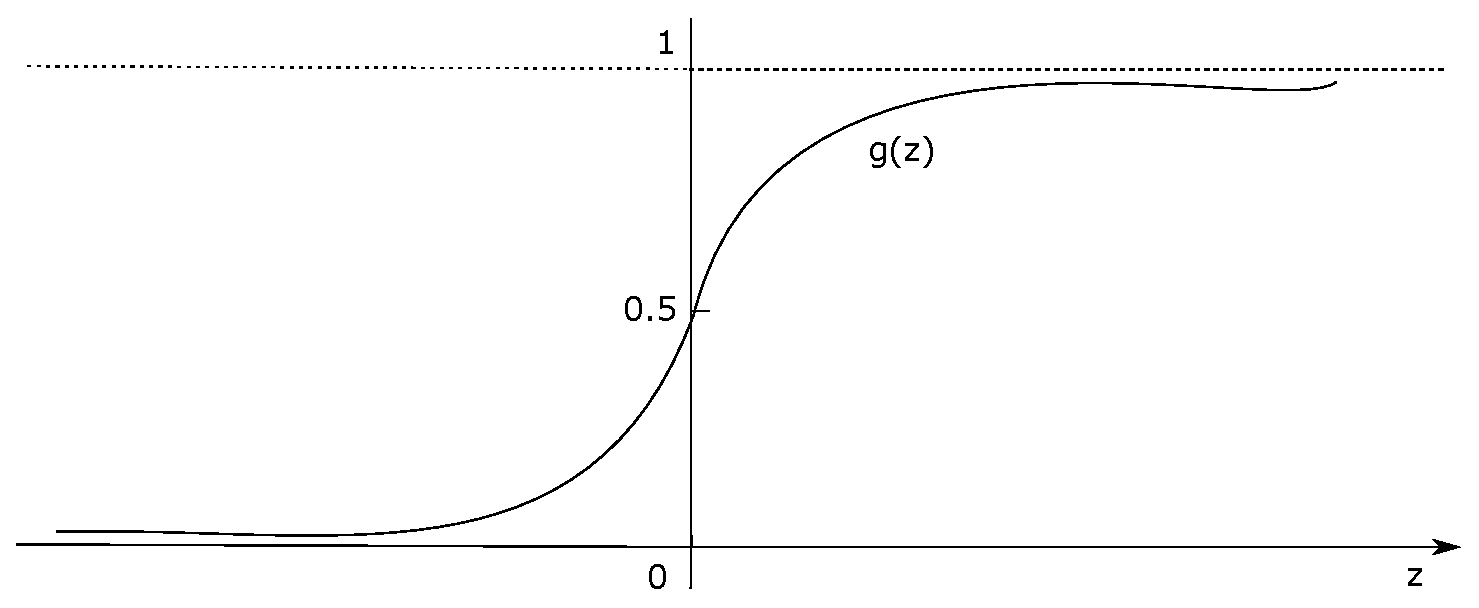
\includegraphics[height = 1.5in]{ml_images/sigmoid}
\end{center}

As we see on the plot, the sigmoid function maps any real number to the $(0, 1)$ interval, making it useful for transforming an arbitrary-valued function into a function better suited for classification.

\subsection*{Decision boundaries}

The equation \eqref{eq:log-reg-hyp} gives $h_\theta(x)$ as the estimated probability that $y=1$ given the input $x$ and the parameters $\theta$, so to get our binary classification, we can translate the output of the hypothesis function as follows:

\begin{align*}
  h_\theta(x) \geq 0.5 & \longrightarrow y =1 \\
  h_\theta(x) < 0.5 & \longrightarrow y = 0
\end{align*}

Since $h_\theta(x) = g(\theta^Tx)$, and looking on how $g$ behaves on positive/negative numbers, we observe that $$h_\theta(x) = g(\theta^T x) \geq 0.5  \text{, if } \theta^T x \geq 0$$ and $$h_\theta(x) = g(\theta^T x) < 0.5  \text{, if } \theta^T x < 0.$$

Therefore:

\begin{align*}
  \theta^Tx \geq 0 & \longrightarrow y =1 \\
  \theta^Tx < 0 & \longrightarrow y = 0
\end{align*}

The line defined by $\theta^Tx = 0$ is called "decision boundary" and separates the area where $y = 0$ and where $y = 1$. Note that it depends only on the hypothesis function.

\textbf{TODO:}
\begin{itemize}
  \item add image with decision boundary
\end{itemize}

In general, we can consider more complex decision boundaries (polynomial, etc.) depending on the initial hypothesis we plug into the sigmoid function. For example, if we take \break
$z = \theta_0 + \theta_1x_1^2 +\theta_2x_2^2$, then the decision boundary $\theta_0 + \theta_1x_1^2 +\theta_2x_2^2 = 0$ is a circle.

\subsection*{Cost function}

 We cannot use the same cost function that we use for linear regression because the logistic function will cause the output to have many local optima (in other words, it will not be a convex function).

Instead, we define the cost function for logistic regression as:

\begin{equation}\label{eq:log-reg-cost}
J(\theta) = \dfrac{1}{m} \sum_{i=1}^{m}{\cost(h_\theta(x^i), y^i)},
\end{equation}
where the cost of a single training example is given by:

$$\cost(h_\theta(x), y) = \left\{\begin{matrix}
                                    -\log(h_\theta(x)) & \text{, if } y = 1 \\
                                    -\log(1 - h_\theta(x)) & \text{, if } y = 0
                                  \end{matrix}\right.$$

This new cost function, defined by equation \eqref{eq:log-reg-cost}, is convex so we can apply gradient descent to find the optimal $\theta$.

\hspace{1.0in}

\begin{center}
\begin{minipage}{0.48\textwidth}
 \centering
 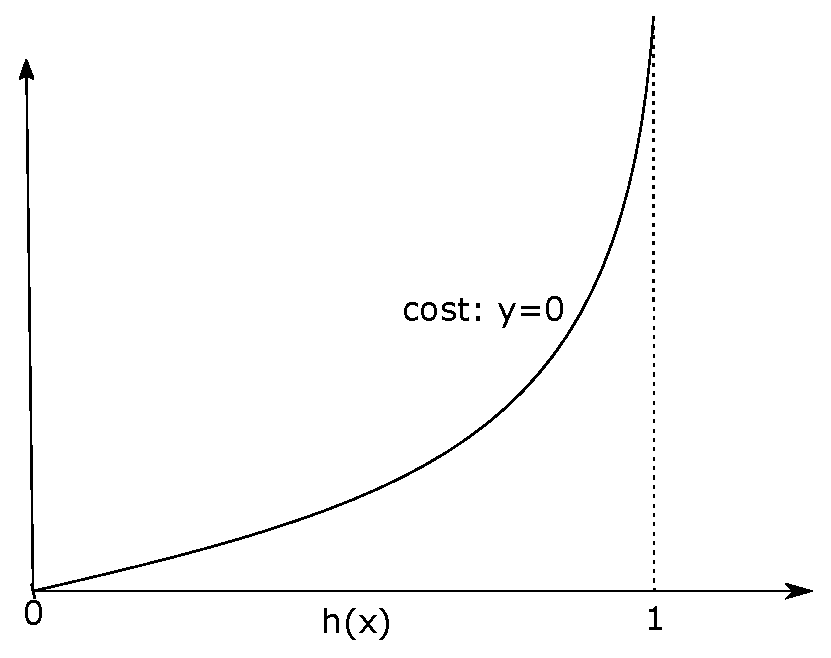
\includegraphics[width=.8\linewidth]{ml_images/cost_0}
 %\captionof*{figure}{Cost when y = 0}
\end{minipage}\hfill
\begin{minipage}{0.48\textwidth}
 \centering
 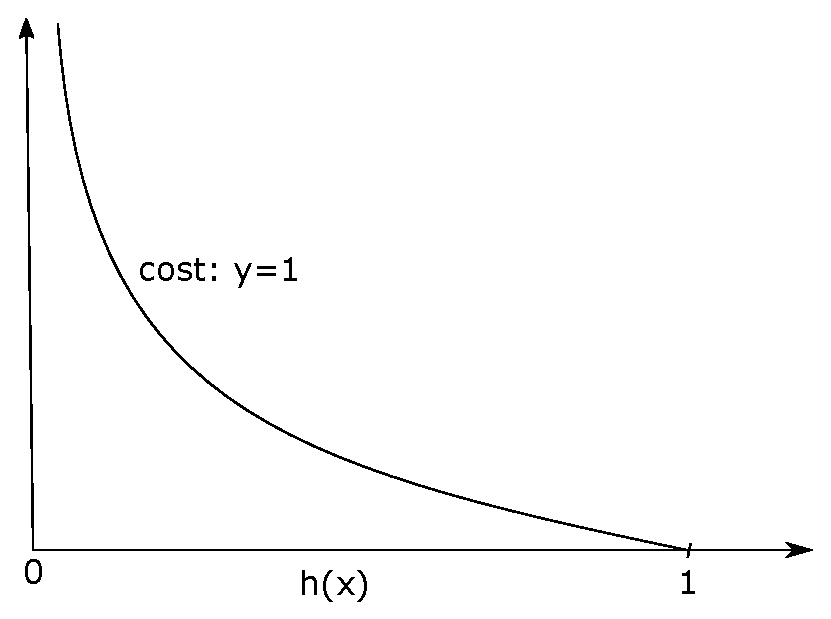
\includegraphics[width=.8\linewidth]{ml_images/cost_1}
 %\captionof*{figure}{Cost when y = 1}
\end{minipage}
\end{center}

Note that if $y = 1$ and $h_\theta(x) = 1$, then the $\cost$ will be $0$. If $y = 1$ and $h_\theta(x) \longrightarrow 0$ , then $\cost\longrightarrow \infty$, so wrong predictions are penalized by a very large cost (see figures).

\subsection*{Gradient descent}

 We can compress the cost function's two conditional cases into one case: $$\cost(h_\theta(x),y) = - y \; \log(h_\theta(x)) - (1 - y) \log(1 - h_\theta(x))$$

Notice that when $y$ is equal to $1$, then the second term $(1-y)\log(1-h_\theta(x))$ will be zero and will not affect the result. If $y$ is equal to $0$, then the first term $-y \log(h_\theta(x))$ will be zero and will not affect the result.

We can fully write out the cost function as follows:
\begin{equation}\label{eq:log-reg-cost2}
J(\theta) = - \frac{1}{m} \displaystyle \sum_{i=1}^m [y^{i}\log (h_\theta (x^{i})) + (1 - y^{i})\log (1 - h_\theta(x^{i}))],
\end{equation}
or vectorized as:
\begin{equation}\label{eq:log-reg-cost-vec}
J(\theta)  = \frac{1}{m} \left(-y^{T}\log(h)-(1-y)^{T}\log(1-h)\right),
\end{equation}
where $h = g(X\theta)$.

Remember the general form of gradient descent, as in \eqref{eq:lin-reg-gd}: $$\theta_j := \theta_j - \alpha \dfrac{\partial}{\partial \theta_j}J(\theta).$$

Computing the partial derivative for the cost function \eqref{eq:log-reg-cost2}, it turns out that the gradient decent equations for logistic regression look exactly the same as for linear regression:
$$\theta_j := \theta_j - \frac{\alpha}{m} \sum_{i=1}^m (h_\theta(x^{i}) - y^{i}) x_j^{i}.$$

A vectorized implementation of the gradient descent is given by: $$\theta := \theta - \frac{\alpha}{m} X^{T} (g(X \theta ) - {y}).$$

\section*{Stochastic Gradient Descent}

Stochastic gradient descent is an alternative to batch gradient descent (where all the training examples are used in one iteration) and is more efficient and scalable to large data sets.

The cost of one training example is:

$$cost(\theta,(x^{(i)}, y^{(i)})) = \dfrac{1}{2}(h_{\theta}(x^{(i)}) - y^{(i)})^2.$$

The cost of the training set is:

$$J_{train}(\theta) = \dfrac{1}{m} \displaystyle \sum_{i=1}^m cost(\theta, (x^{(i)}, y^{(i)})).$$

First, randomly shuffle the dataset. Then for $i = 1\dots m$:
$$\Theta_j := \Theta_j - \alpha (h_{\Theta}(x^{(i)}) - y^{(i)}) \cdot x^{(i)}_j$$

The algorithm fits one training example at a time. This way we can make progress in gradient descent without having to scan all $m$ training examples first. Stochastic gradient descent is unlikely to converge at the global minimum and will instead wander around it randomly, but usually yields a result that is close enough. Stochastic gradient descent usually takes 1-10 passes through your data (epochs) set to get near the global minimum.

\section*{Mini-Batch Gradient Descent}

Mini-batch gradient descent can sometimes be even faster than stochastic gradient descent. Instead of using all $m$ examples as in batch gradient descent, and instead of using only 1 example as in stochastic gradient descent, we will use some in-between number of examples $b$.

Typical values for $b$ range from 2-100 or so.

For example, with $b=10$ and $m=1000$:

Repeat:

For $i = 1,11,21,31,\dots,991$

$$\theta_j := \theta_j - \alpha \dfrac{1}{10} \displaystyle \sum_{k=i}^{i+9} (h_\theta(x^{(k)}) - y^{(k)})x_j^{(k)}$$

We're simply summing over ten examples at a time. The advantage of computing more than one example at a time is that we can use vectorized implementations over the b examples.

\section*{Stochastic Gradient Descent Convergence}

How do we choose the learning rate $\alpha$ for stochastic gradient descent? Also, how do we debug stochastic gradient descent to make sure it is getting as close as possible to the global optimum?

One strategy is to plot the average cost of the hypothesis applied to every 1000 or so training examples. We can compute and save these costs during the gradient descent iterations.

With a smaller learning rate, it is possible that you may get a slightly better solution with stochastic gradient descent. That is because stochastic gradient descent will oscillate and jump around the global minimum, and it will make smaller random jumps with a smaller learning rate.

If you increase the number of examples you average over to plot the performance of your algorithm, the plot's line will become smoother.

With a very small number of examples for the average, the line will be too noisy and it will be difficult to find the trend.

One strategy for trying to actually converge at the global minimum is to slowly decrease $\alpha$ over time. However, this is not often done because people don't want to have to fiddle with even more parameters.

\subsection*{Multiclass classification: one-vs-all}

Assume that we have more than two classes in the classification problem, i.e. instead of having $y = \{0,1\}$, we have $y = \{0,1, \ldots, k\}$, with $k \geq 3$.
In this case, we divide the problem into $k+1$ binary classification problems; in each one, we predict the probability that $y$ is a member of one of the classes.

We have $k+1$ hypotheses $h_\theta^{(0)}, h_\theta^{(1)}, \ldots, h_\theta^{(k)}$, defined as:
\begin{align*}
h_\theta^{(0)}(x) &= \mathbb{P}(y = 0 | x ; \theta), \\
h_\theta^{(1)}(x) &= \mathbb{P}(y = 1 | x ; \theta), \\
\vdots &\\
h_\theta^{(k)}(x) &= \mathbb{P}(y = n | x ; \theta), \\
\end{align*}
and we make the final prediction by taking:

$$h_\theta(x) := \max_{i\leq k} h_\theta ^{(i)}(x). \\$$

We basically choose one class and then lump all the others into a single second class. We do this repeatedly, applying binary logistic regression to each case, and then use the hypothesis that returned the highest value as our prediction.


\section{Regularization}

\subsubsection*{Overfitting/underfitting}

High bias or underfitting is when the form of our hypothesis function $h$ maps poorly to the trend of the data. It is usually caused by a function that is too simple or uses less features, e.g. if we take
$h_\theta(x) = \theta_0 + \theta_1x_1 + \theta_2x_2$ then we make an initial assumption that a linear model fits the training data well and will be able to generalize but that may not be the case.

At the other extreme, overfitting or high variance is caused by a hypothesis function that fits the available data but does not generalize well to predict new data. It is usually caused by a complicated function that creates a lot of unnecessary curves and angles unrelated to the data.

This terminology is applied to both linear and logistic regression. There are two main options to address the issue of overfitting:
\begin{itemize}
\item reduce the number of features:
    \begin{itemize}
      \item manually select which features to keep,
      \item use a model selection algorithm.
    \end{itemize}

\item regularization: keep all the features, but reduce the size of the parameters $\theta_j$.
\end{itemize}
Regularization is designed to address the problem of overfitting and works well when we have a lot of slightly useful features.

If the hypothesis function overfits the data, we can reduce the weight that some of the terms in the function carry by increasing their cost. Assume we have the following hypothesis:
$\theta_0 + \theta_1x + \theta_2x^2 + \theta_3x^3 + \theta_4x^4$ and we want to make it more quadratic, i.e. we want to eliminate the influence of $\theta_3x^3$ and $\theta_4x^4$.

Instead of getting rid of these features or changing the form of the hypothesis, we can modify the cost function as such:

$$J(\theta) = \ds \dfrac{1}{2m}\sum_{i=1}^m (h_\theta(x^i) - y^{i})^2 + 1000\cdot\theta_3^2 + 1000\cdot\theta_4^2.$$

We add two extra terms at the end to inflate the cost of $\theta_3$ and $\theta_4$. Now, in order for the cost function to get close to zero, we have to reduce the values of $\theta_3$ and $\theta_4$ to near zero. This will in turn greatly reduce the values of $\theta_3x^3$ and $\theta_4x^4$ in our hypothesis function.

We can regularize all parameters at once and define a regularized cost function as:

\begin{equation}\label{eq:reg-cost}
J(\theta) = \ds \dfrac{1}{2m} \left[ \sum_{i=1}^m (h_\theta(x^{i}) - y^{i})^2 + \lambda \sum_{j=1}^n \theta_j^2 \right],
\end{equation}
where $\lambda > 0$ is the regularization parameter. By convention, the parameter $\theta_0$ is not regularized.

In fact $\lambda$ represents a trade-off between a good fit of the data and smaller parameters (a simpler hypothesis). If $\lambda$ is chosen to be too large, it may simplify the hypothesis too much and cause underfitting. Observe that the regularization term is actually equal to $\lambda \norm{\theta}_2^2$, where $\theta^T = [\theta_1, \ldots, \theta_n]$. One can also regularize by the term $\lambda \norm{\theta}_1^2$, and even by a combination of them: $\lambda_1 \norm{\theta}_1^2 + \lambda_2 \norm{\theta}_2^2$.

\subsection*{Regularized linear regression}

Assume that we regularize the cost function for linear regression as in \eqref{eq:reg-cost}. Then the gradient descent equations become:

\begin{equation}\label{eq:mul-reg-gdreg}
\begin{split}
\theta_0 := & \; \theta_0 - \alpha \dfrac{1}{m} \sum_{i=1}^m (h_\theta(x^{i}) - y^{i})x_0^{i}, \\
\theta_j := & \; \theta_j - \alpha \left[ \left( \dfrac{1}{m}\sum_{i=1}^m (h_\theta(x^{i}) - y^{i})x_j^{i} \right) + \frac{\lambda}{m}\theta_j \right], \; j\geq 2. \\
\end{split}
\end{equation}

Recall that $\theta$ can be also obtained as a solution of the normal equation \eqref{eq:mul-reg-neq}: $$\theta = (X^TX)^{-1}X^Ty.$$

One can prove that the regularized normal equation becomes: $$\theta = (X^TX +\lambda \cdot I)^{-1}X^Ty,$$
where $I$ is a $(n+1)\times (n+1)$ diagonal matrix with entries $(0,1,1,\ldots, 1)$. Actually, $I$ is very similar to the identity matrix $I_{n+1}$ except for the $(1,1)$ entry which is 0 in our case, since $\theta_0$ is not regularized.

We mentioned before that $X^TX$ may not be invertible if $m \leq n$. However, by adding the regularization term $\lambda\cdot I$, the matrix $X^TX +\lambda\cdot I$ becomes invertible.

\subsection*{Regularized logistic regression}

We can regularize logistic regression in a similar way as linear regression. Let's start with the regularized cost function:

\begin{equation}\label{eq:log-reg-costreg}
J(\theta) = - \dfrac{1}{m} \sum_{i=1}^m [ y^{i}\log (h_\theta (x^{i})) + (1 - y^{i}) \log (1 - h_\theta(x^{i}))\large] + \frac{\lambda}{2m}\sum_{j=1}^n \theta_j^2
\end{equation}
​	
The gradient descent equations are identical to \eqref{eq:mul-reg-gdreg}:

\begin{equation*}
\begin{split}
\theta_0 := & \; \theta_0 - \alpha \dfrac{1}{m} \sum_{i=1}^m (h_\theta(x^{i}) - y^{i})x_0^{i}, \\
\theta_j := & \; \theta_j - \alpha \left[ \left( \dfrac{1}{m}\sum_{i=1}^m (h_\theta(x^{i}) - y^{i})x_j^{i} \right) + \frac{\lambda}{m}\theta_j \right], \; j\geq 2. \\
\end{split}
\end{equation*}

\textbf{TODO:}
\begin{itemize}
  \item ridge/lasso/elastic net regression
  \item lasso regression as feature selection method
\end{itemize}


\chapter{Neural Networks}

\section{Neural networks representation}

\subsection*{Non-linear hypotheses}

Performing linear regression with a complex set of data and many features is very unwieldy. Assume that we have 3 features and want to define a hypothesis that includes all the quadratic terms:
$$g(\theta_0 + \theta_1x_1^2 + \theta_2x_1x_2 + \theta_3x_1x_3 + \theta_4x_2^2 + \theta_5x_2x_3 + \theta_6x_3^2).$$

That gives us 6 features. If we start with 100 features and want to include all the quadratic terms, we get $5050$ resulting features.

One can approximate the growth of the number of new features we get with all quadratic terms with $\mathcal{O}({n^2}/{2})$. If we want to include all cubic terms in our hypothesis, the number of features grows asymptotically at $\mathcal{O}(n^3)$. These are very steep growths, so as the number of our features increase, the number of quadratic or cubic features increase very rapidly and becomes quickly impractical.

For example, assume that the training set is a collection of $50 \times 50$ pixel B\&W photographs, and our goal will be to classify which ones are photos of cars. Our feature set size is then $n = 2500$ if we compare every pair of pixels. Now let's say we consider a quadratic hypothesis function. In this case, the total number of features will be about $2500^2 / 2 = 3125000$, which is very impractical.

Neural networks offers an alternate way to perform machine learning when we have complex hypotheses with many features.

\subsection*{Model representation}

At a very simple level, brain neurons are computational units that take input (dendrites) as electrical input which is channeled to outputs (axons).

We start from logistic regression and build an abstract representation of a neuron (also called logistic unit in this context). The inputs (dendrites) are the features $x_1, \ldots, x_n$, and the output (axon) is the result of the hypothesis function $h_\theta(x) = g(\theta^Tx)$. The components of a layer are called nodes or units.

\begin{center}
\begin{neuralnetwork}[height=4]
    \newcommand{\x}[2]{$x_#2$}
    \newcommand{\h}[2]{$h_\theta$}
    \newcommand{\ab}[2]{$z$}
    \newcommand{\linktheta}[4]{$\theta_#2$}
    \newcommand{\linkg}[4]{$g$}
    \inputlayer[count=2, bias=true, title=Input layer, text=\x]
    \outputlayer[count=1, text=\ab]
    \setdefaultlinklabel{\linktheta}
    \linklayers
    \outputlayer[count=1, title=Output, text=\h]
    \setdefaultlinklabel{\linkg}
    \linklayers
\end{neuralnetwork}
\captionof*{figure}{Neuron model (logistic unit)}
\end{center}

As before, we add an extra input node $x_0 = 1$, which is called "bias unit". The parameters $\theta_0, \theta_1, \ldots, \theta_n$ are now called "weights". We compute the output of the node $z$ by taking the weighted sum of the inputs, i.e. $z = \theta^Tx = \theta_0x_0 + \theta_1x_1 + \ldots + \theta_nx_n$.

To get the actual output $h_\theta(x)$ we apply the logistic (or sigmoid) function $g(z) = \dfrac{1}{1+\mathrm{e}^{-z}}$ to the node $z$ ($g$ is called the "activation function" of the node $z$), hence:
$$ h_\theta(x) = g(\theta^Tx) = \dfrac{1}{1 + \mathrm{e}^{-\theta^Tx}}.$$

One can use other functions with similar properties as activation functions.

The first layer is called the "input layer" and the final layer the "output layer," which gives the final value computed by the hypothesis. We can have intermediate layers of nodes between input and output, called "hidden layers." The nodes of a hidden layer are also called "activation units".

\begin{center}
\begin{neuralnetwork}[height=4]
    \newcommand{\x}[2]{$x_#2$}
    \newcommand{\au}[2]{$a^{#1}_#2$}
    \newcommand{\weights}[4]{$\theta^#3_{#4#2}$}
    % from layer=#1, from node=#2 to layer=#3, to node=#4
    \setdefaultlinklabel{\weights}
    \inputlayer[count=3, bias=true, title=Input, text=\x]
    \hiddenlayer[count=3, bias=true, title=Hidden, text=\au]
    \linklayers[title=$\Theta^1$]
    \outputlayer[count=1, title=Output, text=\au]
    \linklayers[title=$\Theta^2$]
\end{neuralnetwork}
\captionof*{figure}{Network with one hidden layer}
\end{center}

This figure describes a simple neural network with one hidden layer. The input layer has three units $x_1, x_2, x_3$, plus the bias unit $x_0=1$. The hidden layer has three nodes $a^1_1, a^1_2, a^1_3$, and as before we add a bias node $a^1_0=1$. Finally, we have one output node $a^2_1 = h_\Theta(x)$.

To map the input layer to the hidden layer we use a matrix of weights $\Theta^1 = \{\theta^1_{ik}\}\in\mathbb{R}^{3\times 4}$, where $k$ represents the starting node and $i$ represents the target node. Similarly, to map the hidden layer to the output layer we use a matrix of weights $\Theta^2 = \{\theta^2_{ik}\}\in\mathbb{R}^{1\times 4}$.

The values of the activation units $a^j_i$ are computed as follows:

\begin{equation}\label{eq:nn-act-nod}
\begin{split}
a_1^{1} = & g(\theta_{10}^{1}x_0 + \theta_{11}^{1}x_1 + \theta_{12}^{1}x_2 + \theta_{13}^{1}x_3), \\
a_2^{1} = & g(\theta_{20}^{1}x_0 + \theta_{21}^{1}x_1 + \theta_{22}^{1}x_2 + \theta_{23}^{1}x_3), \\
a_3^{1} = & g(\theta_{30}^{1}x_0 + \theta_{31}^{1}x_1 + \theta_{32}^{1}x_2 + \theta_{33}^{1}x_3), \\
h_\theta(x) =  a_1^{2} = & g(\theta_{10}^{2}a_0^{1} + \theta_{11}^{2}a_1^{1} + \theta_{12}^{2}a_2^{1} + \theta_{13}^{2}a_3^{1}). \\
\end{split}
\end{equation}

The process of computing the values of all nodes starting from the input units is called "forward propagation".

Let's fix some notations we are going to use from now on:
\begin{align*}
x_i = & \text{ the input units, including the bias unit }, \\
s_j = & \text{ the number of units in layer $j$}, \\
a_i^j = & \text{ activation of unit $i$ in layer $j$}, \\
\Theta^j = & \text{ matrix of weights mapping layer $j-1$ to layer $j$}.
\end{align*}

Since we have $s_{j-1}$ units in layer $j-1$ and $s_{j}$ units in layer $j$, then the dimension of the matrix $\Theta^j$  is $s_{j}\times (s_{j-1}+1)$. The $+1$ comes from the addition of the bias nodes in the input.

\subsection*{Vectorized representation}

In this section we describe a vectorized implementation of the forward propagations equations.
Assume we have $n$ input nodes and one hidden layer as the network in the previous figure. We denote by $z^j_i$ the inputs of function $g$ in equations \eqref{eq:nn-act-nod}. More precisely:

\begin{equation}\label{eq:nn-def-z's}
\begin{split}
z_i^{1} = & \; \theta_{i0}^{j}x_0 + \theta_{i1}^{1}x_1 + \cdots + \theta_{in}^{1}x_n,\; i=1,\ldots,n, \\
z_1^{2} = & \; \theta_{10}^{2}a_0^{1} + \theta_{11}^{2}a_1^{1} + \theta_{12}^{2}a_2^{1} + \theta_{13}^{2}a_3^{1}. \\
\end{split}
\end{equation}

Considering vectors $x = [x_0, x_1, \ldots, x_n]^T$ and $z^j = [z^j_1, z^j_2, \ldots, z^{j}_{s_j}]^T$  and $x = a^0$, we can write: $$z^{j} = \Theta^{j} \cdot a^{j-1}, \; \text{ for each layer } j.$$

Recall that the matrix $\Theta^j$ has dimension $s_{j}\times (s_{j-1}+1)$, where $s_j$ is the number of activation nodes in layer $j$. The vector $a^{j-1}$ has $s_{j-1}+1$ elements, so the resulting vector $z^{j}$ has $s_j$ elements.

Having this in hand, we can write the activation nodes for layer $j$ as follows: $$a^{j} = g(z^{j}),$$ where $g$ is applied element-wise to the vector $z^{j}$. After computing $a^{j}$, we then add a bias unit $a_0^{j} = 1$ to layer $j$.

If $j+1$ is the output layer, to compute our hypothesis, we first have: $$z^{j+1}=\Theta^{j+1}\cdot a^j.$$
Since $\Theta^{j+1}$ has dimension $s_{j+1}\times (s_{j}+1)$, $a^j$ has $s_j + 1$ elements and $s_{j+1} = 1$, we get that $z^{j+1}$ is just a real number.
Finally: $$h_\Theta(x) = a^{j+1} = g(z^{j+1}).$$


\subsubsection*{Example 1}

A simple example of applying neural networks is by predicting the output of a logical operator \verb"AND" which returns \verb"TRUE" if and only if both arguments are \verb"TRUE".

We use a simple network with no hidden layers:

\begin{center}
\begin{neuralnetwork}[height=4]
    \newcommand{\x}[2]{$x_#2$}
    \newcommand{\h}[2]{$h_\theta(x)$}
    \inputlayer[count=2, bias=true, text=\x]
    \outputlayer[count=1, text=\h]
    \linklayers[title=$\theta^1$]
\end{neuralnetwork}
\end{center}

Remember that $x_0$ is the bias input and is always equal to 1. Setting $$\theta^1 := [−30, 20, 20],$$ we have: $$h_\Theta(x) = g(-30 + 20x_1 + 20x_2).$$

More explicitly, we get the following cases:
\begin{align*}
x_1 = 0 \text{ and } x_2 = 0  \longrightarrow h_\theta(x) = &\; g(-30) \sim 0 \\
x_1 = 0 \text{ and } x_2 = 1  \longrightarrow h_\theta(x) = &\; g(-10) \sim 0 \\
x_1 = 1 \text{ and } x_2 = 0  \longrightarrow h_\theta(x) = &\; g(-10) \sim 0 \\
x_1 = 1 \text{ and } x_2 = 1  \longrightarrow h_\theta(x) = &\;\;\;\; g(10)  \sim 1 \\
\end{align*}
So we have built one of the fundamental operations in computers by using a small neural network rather than using an actual \verb"AND" gate.

\subsubsection*{Example 2}

Neural networks can also be used to simulate all the other logical gates. The weights matrix for \verb"OR"  is $[-10, 20, 20]$ and for \verb"NOR" is $[10, -20, -20]$.
We can combine these to get the \verb"XNOR" logical operator, which returns 1 if $x_1$ and $x_2$ are both 0 or both 1.

\begin{center}
\begin{neuralnetwork}[height=4]
    \newcommand{\x}[2]{$x_#2$}
    \newcommand{\au}[2]{$a^{#1}_#2$}
    \newcommand{\h}[2]{$h_\theta(x)$}
    \inputlayer[count=2, bias=true,text=\x]
    \hiddenlayer[count=2, bias=true, text=\au]
    \linklayers[title=$\theta^1$]
    \outputlayer[count=1, text=\h]
    \linklayers[title=$\theta^2$]
\end{neuralnetwork}
\end{center}

To map the input layer to the hidden layer, we use a $\theta^1$ matrix that combines the values for \verb"AND" and \verb"NOR":
$$\Theta^{(1)} =\begin{bmatrix}-30 & 20 & 20 \\ 10 & -20 & -20\end{bmatrix}.$$

To map the hidden layer to the output layer, we use the $\Theta^2$ matrix of \verb"OR": $$\Theta^{(2)} =\begin{bmatrix}-10 & 20 & 20\end{bmatrix}.$$

One can easily check that this simple network with one hidden layer indeed implements the operator \verb"XNOR".

\subsection*{Multiclass Classification}

To classify a set of data into multiple classes, we allow our hypothesis function to return a vector of values. Assume that we want to classify our data into one of the four resulting classes:

\begin{center}
\begin{neuralnetwork}[height=5.5]
    \newcommand{\x}[2]{$x_#2$}
    \newcommand{\au}[2]{$a^{#1}_#2$}
    \newcommand{\h}[2]{${h_\theta}_#2$}
    %\newcommand{\weights}[4]{$\theta^#3_{#4#2}$}
    % from layer=#1, from node=#2 to layer=#3, to node=#4
    %\setdefaultlinklabel{\weights}
    \inputlayer[count=5, bias=true, title=Input, text=\x]
    \hiddenlayer[count=4, bias=true, title=Hidden, text=\au] \linklayers
    \hiddenlayer[count=4, bias=true, title=Hidden, text=\au] \linklayers
    \outputlayer[count=4, title=Output, text=\h] \linklayers
\end{neuralnetwork}
\captionof*{figure}{Network with many hidden layer}
\end{center}

The final hidden layer, when multiplied by its $\theta$ matrix, will map to a vector on which we apply the sigmoid function $g$ or other activation function to get the final vector of hypothesis values.


\section{Neural networks learning}

\textbf{TODO:} fix convention for weights matrix $\theta$ or $\Theta$ + better notations.

\subsection*{Cost function}

Remember from the previous section that, for a neural network, we denote by $L$ total number of layers in the network, by $s_j$ the number of units (not counting the bias unit) in layer $j$ and by $K \geq 1$ the number of output units/classes. We denote by $h_\theta(x)_k$ the hypothesis that results in the $k$-th output.

We have seen in the previous section that a neural network looks locally like a logistic regression. The cost function we use for training neural networks is going to be a generalization of the cost function for logistic regression. Recall from \eqref{eq:log-reg-costreg} the cost function for regularized logistic regression:
$$ J(\theta) = - \dfrac{1}{m} \sum_{i=1}^m \large[ y^{i}\ \log (h_\theta (x^{i})) + (1 - y^{i})\ \log (1 - h_\theta(x^{i}))\large] + \frac{\lambda}{2m}\sum_{j=1}^n \theta_j^2.$$

For neural networks, the cost function is going to be slightly complicated:

\begin{equation}\label{eq:nn-cost}
\begin{split}
J(\Theta) = & - \dfrac{1}{m} \sum_{i=1}^m \sum_{k=1}^K \left[y^{i}_k \log ((h_\Theta (x^{i}))_k) + (1 - y^{i}_k)\log (1 - (h_\Theta(x^{i}))_k)\right] + \\
            & + \dfrac{\lambda}{2m}\sum_{l=1}^{L-1} \sum_{i=1}^{s_{l-1}} \sum_{j=1}^{s_{l}} \left( \Theta_{ji}^{l}\right)^2
\end{split}
\end{equation}

The first part of the equation \eqref{eq:nn-cost} looks similar to \eqref{eq:log-reg-costreg}, and additionally  we sum up over $K$, the number of the output nodes.

The regularization term includes all the weights that appear along the network. Recall that the dimension of $\Theta^l$ is $s_l \times (s_{l-1}+1)$, but since we do not regularize the bias weights, we actually have that $\Theta^l$ is $s_l \times (s_{l-1})$ dimensional.


\subsection*{The backpropagation algorithm}

The backpropagation algorithm is a method of computing the partial derivatives of the cost function of a neural network, to use further in gradient descent. Our goal is to find an optimal set of weights $\Theta$ that minimizes the cost function $J$ from \eqref{eq:nn-cost}.

Recall that for gradient descent we have to compute the partial derivatives $\dfrac{\partial}{\partial\Theta^l_{ji}}J(\Theta)$ and update the parameters accordingly at each iteration.

In the case of backpropagation, we compute the "error" $\delta_j^{l}$ of every node $j$ from layer $l$, starting with the last layer. Recall that $a_j^l$ denotes the activation of unit $j$ in layer $l$.

For the output layer, we have that: $$\delta^{L} = a^{L} - y,$$
where $L$ is the number of layers and $a^{L}$ is the vector of outputs of the activation units of the last layer. So the "error" values for the output layer are simply the differences of the nodes in the output layer and the correct values in $y$.

To get the errors of the layers before the output layer, we use an equation that steps us back from right to left:
$$\delta^{l} = (\Theta^{l+1})^T \delta^{l+1}\ .*\ g^\prime(z^{l}),$$
where $z^l$ is defined by \eqref{eq:nn-def-z's} and $g^\prime$ is the derivative of $g$.
The errors of layer $l$ are calculated by multiplying the errors in the next layer with the matrix of weights of layer $l$. We then multiply this element-wise ($.*$) with the derivative of the activation function $g$ evaluated in $z^l$.

One can prove that the derivative of $g$ can be written as $g^\prime(u) = g(u)\ .*\ (1 - g(u))$. Then the backpropagation equation for nodes in layer $l$ becomes:

\begin{equation}\label{eq:nn-bkprp-eq}
\delta^{l} = (\Theta^{l+1})^T \delta^{l+1}\ .*\ a^{l}\ .*\ (1 - a^{l})\in \mathbb{R}^{s_l+1}.
\end{equation}

Ignoring regularization, one can prove that the partial derivatives of the cost function $J$ are given by:
\begin{equation}\label{eq:nn-cost-deriv}
\dfrac{\partial}{\partial \Theta_{ij}^{l}}{J(\Theta)} = \dfrac{1}{m}\sum_{t=1}^m (a^t)_j^{l-1} (\delta^t)_i^{l}.
\end{equation}

Notice that $\delta^{l+1}$  and $a^{l+1}$ are vectors with $s_{l+1}$ elements. Similarly, $a^{l}$ is a vector with $s_l$ elements. Multiplying them produces a matrix that is $s_{l+1}$ by $s_l$ which is the same dimension as $\Theta^l$. That is, the process produces a gradient term for every element in $\Theta^l$.

We can now take all these equations and put them together into an algorithm.

\subsubsection*{The backpropagation algorithm (to compute the partial derivatives of $J(\Theta)$)}

Assume we have a training set ${(x^1,y^1), \ldots, (x^m,y^m)}$, with $m$ observations.
\begin{description}
\item[Step 1]{Set $\Delta^{l}_{ij}:= 0$, for all indices $l, i, j$.}

\item[Step 2] {For each training example $t$:

\begin{itemize}
\item set $a^{0} := x^{t}$,
\item do forward propagation to compute $a^{l}$, for $l=2,3,\ldots,L$,
\item using $y^{t}$, compute $\delta^{L} = a^{L} - y^{t}$,
\item compute $\delta^{L-1}, \delta^{L-2},\ldots, \delta^{2}$, using the backpropagation equation \eqref{eq:nn-bkprp-eq},
\item update $\Delta^{l}_{ij} := \Delta^{l}_{ij} + a_j^{l-1} \delta_i^{l}$.
\end{itemize}
}
\item[Step 3]{Compute $D^l_{ij} := \dfrac{1}{m}\left(\Delta^l_{ij} + \lambda\theta^l_{ij} \right)$, if $j\neq 0$, and $D^{l}_{ij} := \dfrac{1}{m}\Delta^{l}_{ij}$, if $j = 0$.}

\item[Step 4]{Compute $\dfrac{\partial}{\partial\theta^l_{ji}}J(\theta) = D^l_{ij}$, for all indices $l, i, j$.}
\end{description}

Now we have all necessary ingredients to train a neural network.

\textbf{TODO:} vectorized implementation of gradient descent ?

\subsection*{Training a neural network}

\begin{enumerate}
  \item Choose a network architecture (layers, outputs, units, etc.):
    \begin{itemize}
      \item number of input units = number of features,
      \item number of output units = number of classes,
      \item take one hidden layer as default, or many hidden layers with the same number of units.
    \end{itemize}

  \item Randomly initialize the weights set $\Theta$ (with small values near 0).

  \item Implement forward propagation to compute the output of the hypothesis $h_\Theta$ for all inputs.

  \item Implement the cost function $J(\Theta)$ and implement backpropagation to compute its partial derivatives with respect to all weights $\Theta^l_{ij}$:

    For each training example $(x, y)$:
    \begin{itemize}
      \item do forward propagation to compute the activations $a^l$, for all layers $l$,
      \item do backpropagation to compute the errors $\delta^l$,
      \item update $\Delta^l := \Delta^l + \delta^{l+1}(a^l)^T$ and compute the partial derivatives of $J(\Theta)$.
    \end{itemize}

  \item Use an optimization algorithm (e.g. gradient descent) to find parameters $\Theta$ which minimize the cost function $J(\Theta)$.
\end{enumerate}


\chapter{Model Evaluation}

\section{Evaluating a hypothesis}

A hypothesis may have low error on the training examples, but large error when we try to predict on new examples (because of overfitting). With a given dataset of training examples, we can split up the data into two parts: a training set and a test set, and use them both in the learning process:
\begin{itemize}
\item learn $\theta$ by minimizing $J(\theta)$ on the training set,
\item compute the $J_{\mathrm{test}}(\theta)$ on the test set and compare.
\end{itemize}

For linear regression, the test set error is defined by: $$J_{\mathrm{test}}(\theta) = \dfrac{1}{2m_{\mathrm{test}}}\sum_{i=1}^{m_{\mathrm{test}}}{(h_\theta(x^i_{\mathrm{test}})−y^i_{\mathrm{test}})^2}.$$
For classification problems, we can use the misclassification error:
$$\mathrm{error}(h_\Theta(x),y) =
\left\{\begin{matrix}
1, & \text{ if }  h_\Theta(x) \geq 0.5 \text{ and } y = 0 \text { or } h_\Theta(x) < 0.5  \text{ and } y = 1, \\
0, & \text{ otherwise,}\\
\end{matrix}\right.$$
and then average over the test set:
$$ \text{test error} = \dfrac{1}{m_{\mathrm{test}}} \sum^{m_{\mathrm{test}}}_{i=1} \mathrm{error}(h_\Theta(x^{i}_{\mathrm{test}}), y^{i}_{\mathrm{test}}).$$
This formula gives us the proportion of the test data that was misclassified.

\section{Model selection}

Just because a learning algorithm fits a training set well, that does not mean it is a good hypothesis. The error of a hypothesis as measured on the dataset used to learn the parameters will be lower than on any other dataset.

For example, assume that we have a hypothesis $h_\theta$ which is a polynomial of degree $d$. We can split the initial dataset into training/testing sets and do the following:
\begin{itemize}
  \item optimize $\theta$ on the training set, for each value of $d$,
  \item find the degree $d$ giving the lowest error on the test set,
  \item estimate the generalization error of $h^d_{\theta}$ on the test set.
\end{itemize}
This is a bad method because we learn $d$, the degree of the polynomial hypothesis, using the test set and this will cause the error to be greater for any other set of new data.

To solve this issue, we use an intermediate set to learn $d$, called "cross-validation" set. Typically, we split the initial training set into three parts:
\begin{enumerate}
  \item Training set: $\sim 60\%$ of the data, used to learn several hypotheses $h_\theta$,
  \item Cross-validation set: $\sim 20\%$ of the data, used to test all hypothesis learned and choose the best one,
  \item Testing set: $\sim 20\%$ of the data, used to estimate the generalization error.
\end{enumerate}

\section{Bias vs. Variance}

Most of the time, our models will suffer of one of the following problems (see the figure below):
\begin{description}
  \item[High bias/Underfitting:] the model/hypothesis is too simple to fit the data, and both training and cross-validation error are very high,
  \item[High variance/Overfitting:] the model/hypothesis is too complex, the training error is small and the cross-validation error is large.
\end{description}

\begin{center}
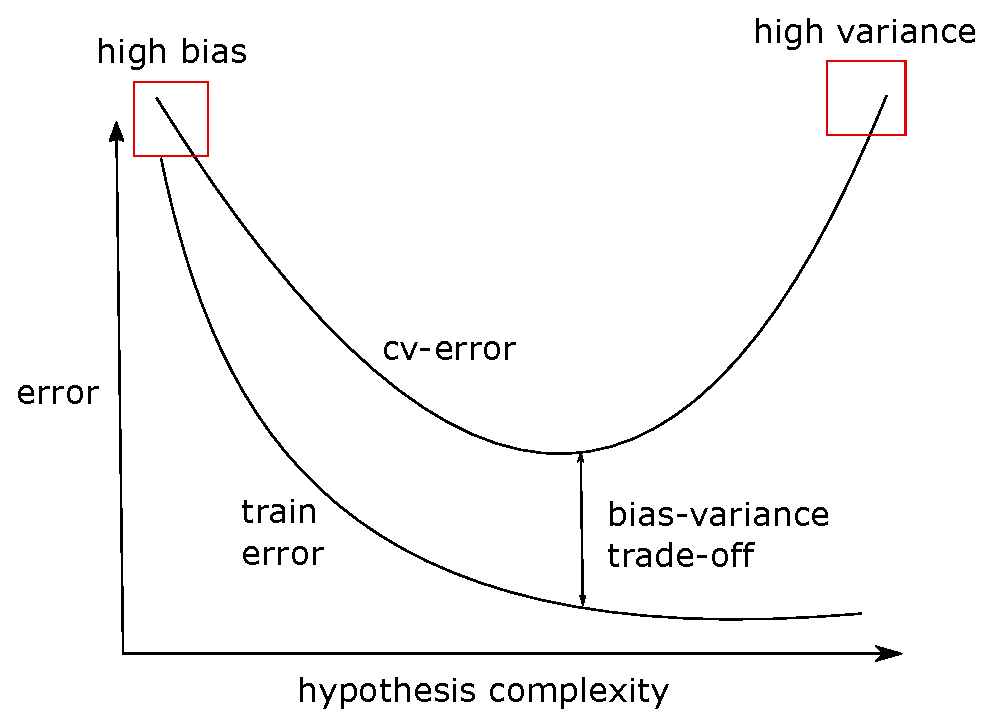
\includegraphics[height = 2in]{ml_images/bias_variance}
\end{center}

If we use a regularized cost function, then choosing a very large parameter $\lambda$ may cause high bias and choosing a very small $\lambda$ may cause high variance. To find the optimal $\lambda$ we use the cross-validation set.

\textbf{TODO:} short explanation of bias-variance trade-off.

\begin{center}
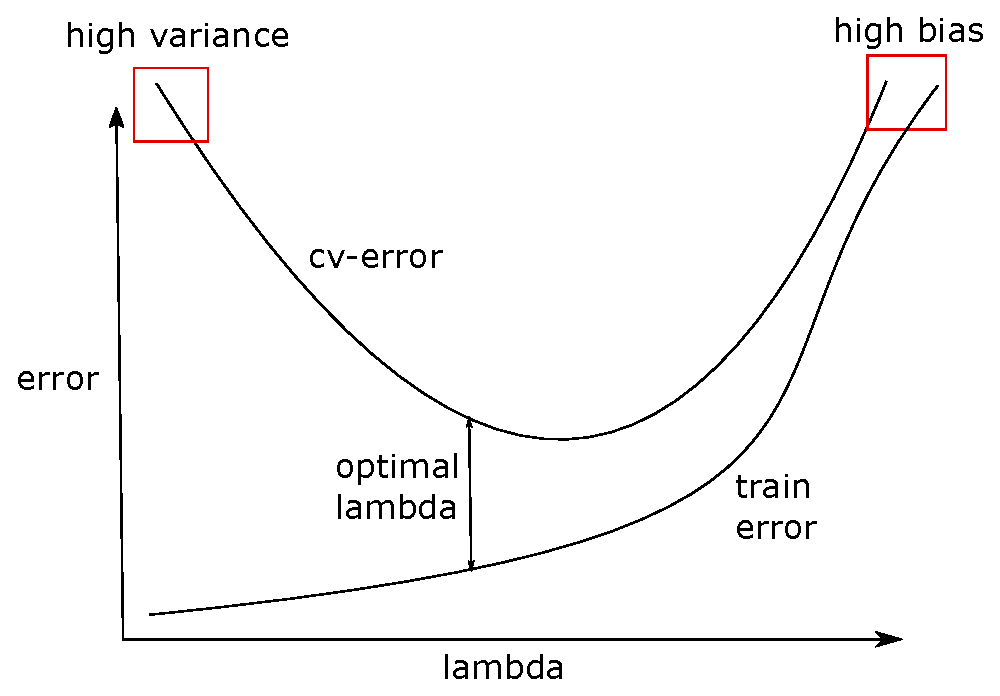
\includegraphics[height = 2in]{ml_images/bias_variance_lambda}
\end{center}

\section{Learning curves}

Training only 3 examples will easily have 0 errors because we can always find a quadratic curve that exactly touches 3 points. As the training set gets larger, the error for a quadratic function increases, but it will flatten  out after a certain $m$. We can observe this by drawing learning curves.
\begin{center}
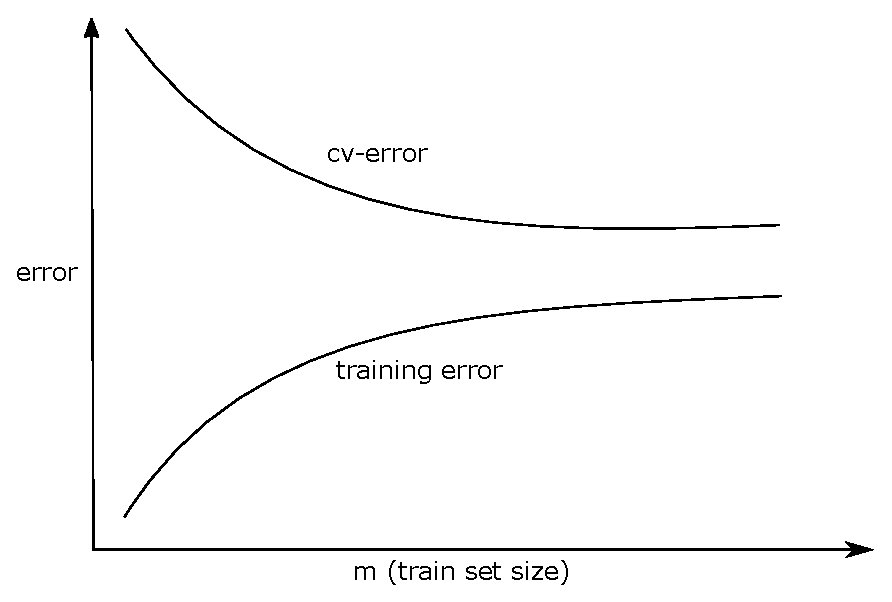
\includegraphics[height = 2in]{ml_images/learn_curve}
\end{center}

If the algorithm suffers from high bias (underfitting), then:
\begin{itemize}
  \item low training set size causes the training error $J_\textrm{train}(\theta)$ to be low and the cross-validation error $J_\textrm{cv}(\theta)$ to be high,
  \item large training set size causes both $J_\textrm{train}(\theta)$ and $J_\textrm{cv}(\theta)$ to be high and very close to each other.
\end{itemize}

\begin{center}
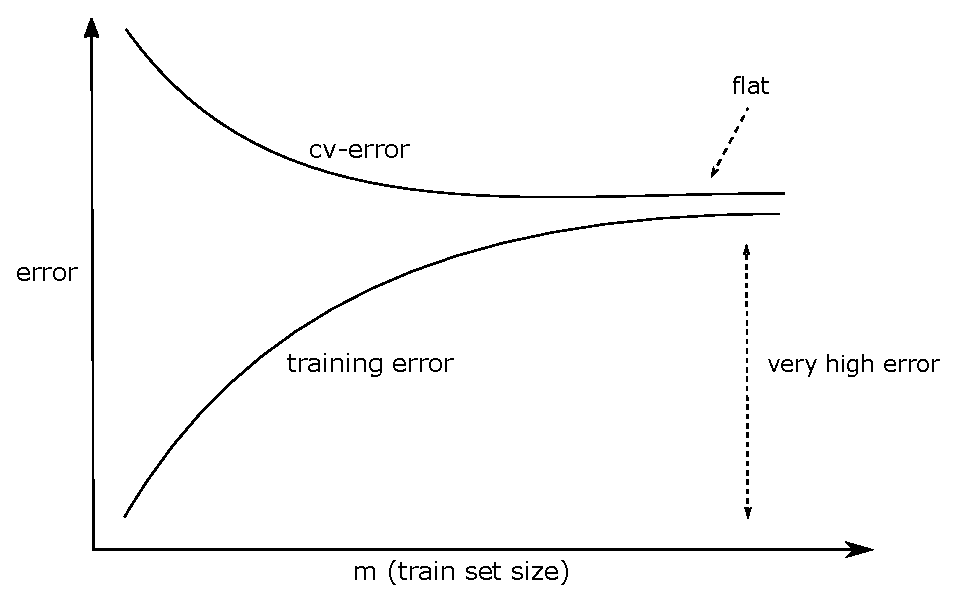
\includegraphics[height = 2in]{ml_images/learn_curve_bias}
\end{center}

If the algorithm suffers from high variance (overfitting), then:
\begin{itemize}
\item low training set size causes low $J_\textrm{train}(\theta)$ and high $J_\textrm{cv}(\theta)$,
\item large training set size makes $J_\textrm{train}(\theta)$ increasing with training set size and $J_\textrm{cv}(\theta)$ decreasing without leveling off (also, $J_\textrm{train}(\theta) < J_\textrm{cv}(\theta)$, but the difference between them remains significant).
\end{itemize}

\begin{center}
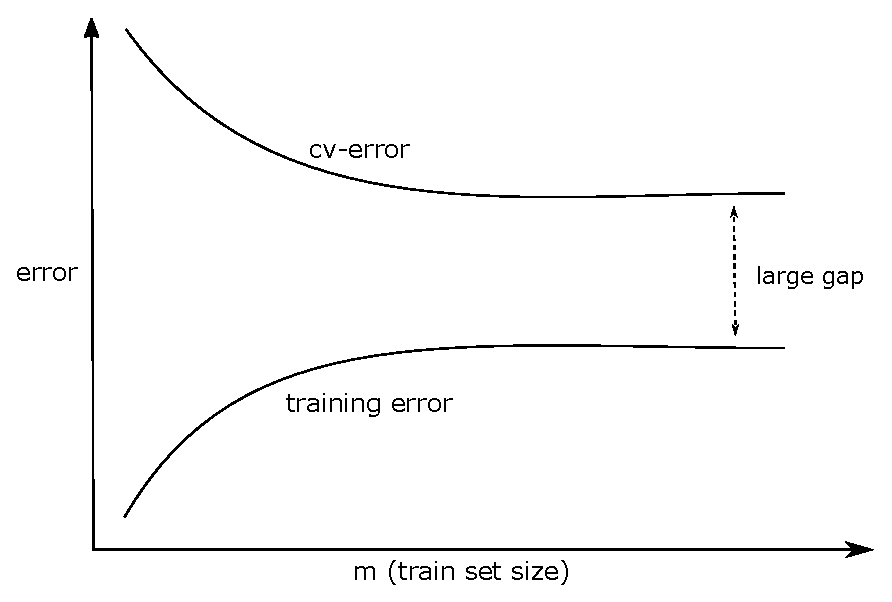
\includegraphics[height = 2in]{ml_images/learn_curve_variance}
\end{center}

Thus, if a learning algorithm is suffering from high bias, getting more training data will not (by itself) help much. On the other hand, in case of high variance, getting more training data is likely to help.

In the case of a neural network, having fewer parameters makes the algorithm prone to underfitting (but it is computationally cheaper). A large neural network with more parameters is prone to overfitting and can be also computationally expensive. If this is the case, we can use regularization to address the overfitting. Using a single hidden layer is a good starting default.

In conclusion, when running model diagnostics we should keep in mind the following things:
\begin{itemize}
\item More training examples fixes high variance but not high bias.
\item Fewer features fixes high variance but not high bias.
\item Additional features fixes high bias but not high variance.
\item The addition of polynomial and interaction features fixes high bias but not high variance.
\item When using gradient descent, decreasing $\lambda$ can fix high bias and increasing $\lambda$ can fix high variance ($\lambda$ is the regularization parameter).
\item When training neural networks, small networks are more prone to underfitting and big networks are prone to overfitting. Cross-validation of network size is a way to choose alternatives.
\end{itemize}

Usually, we start with a simple algorithm, easy to implement, and test it on cross-validation data (quick dirty model). Then we can plot learning curves to decide what comes next: more data, more features, etc. Finally, we do error analysis, i.e. we analyze cross-validation errors to see if anything systematic can be spotted.


\section{Error metrics}

It is sometimes difficult to tell whether a reduction in error is actually an improvement of the algorithm. For example, in predicting a cancer diagnoses where only $0.5\%$ of the examples have cancer, we find a learning algorithm that has a $1\%$ error. However, if we were to simply classify every single example as a 0, then our error would reduce to $0.5\%$ even though we did not improve the algorithm.
This usually happens with skewed classes; that is, when we have a lot more examples from one class than from the other class.

Assume we have a binary classification algorithm, where 1 is the positive class and 0 is the negative class (usually the positive class is the rarest). We use the following terminology for model's predictions:
\begin{description}
  \item[True positive:] Predicted: 1, Actual: 1
  \item[True negative:] Predicted: 0, Actual: 0
  \item[False negative:] Predicted: 0, Actual, 1
  \item[False positive:] Predicted: 1, Actual: 0
\end{description}

The accuracy of the classifier is defined as:
\begin{equation}\label{df:accuracy}
\textrm{Accuracy} = \dfrac{\textrm{True positive} + \textrm{True negative}} {\textrm{Total population}}
\end{equation}

With skewed classes, the accuracy might not be the best metric for deciding the goodness of the classifier, so we also define the precision/recall as:
\begin{equation}\label{df:precision}
\textrm{Precision} = \dfrac{\textrm{True positive}}{\textrm{True positive + False positive}} = \dfrac{\textrm{True positive}}{\textrm{Total predicted positive}},
\end{equation}
i.e. from all predictions with $y=1$, what fraction actually has $y=1$?

\begin{equation}\label{df:recall}
\textrm{Recall} = \dfrac{\textrm{True positive}}{\textrm{True positive + False negative}} = \dfrac{\textrm{True positive}}{\textrm{Total actual positive}},
\end{equation}
i.e. from all examples with $y=1$, what fraction is correctly predicted?

These two metrics give us a better sense of how our classifier is doing. We want both precision and recall to be high. In the example at the beginning of the section, if we classify all patients as 0, then our recall will be $0$, so despite having a lower error percentage, we can quickly see it has worse recall.

If we want to increase the precision (avoid false positives) then one way to do it is to increase the prediction threshold: predict $y=1$ if $h_\theta(x) > 0.7$ for example (this lowers the recall). If we want to increase the recall (avoid false negatives), then we can decrease the prediction threshold, but this is lowering the precision. To trade off these two metrics and encode them into one number, we define the $F_1$ score as their harmonic mean:
\begin{equation}\label{df:F1score}
\textrm{F}_1 \textrm{ score} = 2\cdot \dfrac{\textrm{Precision}\cdot \textrm{Recall}}{\textrm{Precision}+ \textrm{Recall}}
\end{equation}




\chapter{Support vector machines}

\section{SVM with linear kernel}

We describe the optimization objective of a support vector machine (SVM) starting from logistic regression.

Recall that for logistic regression, the hypothesis defined by \ref{eq:log-reg-hyp} is
$$h_\theta(x) = \dfrac{1}{1 + \mathrm{e}^{-\theta^Tx}},$$
and the cost function (optimization objective) defined by \ref{eq:log-reg-cost} is
$$\text{cost}(z) = -y\cdot\log\left(\dfrac{1}{1 + \mathrm{e}^{-z}}\right) - (1-y)\cdot\log\left(1-\dfrac{1}{1 + \mathrm{e}^{-z}}\right),$$
where $z = \theta^Tx$.

Observe that if $y=1$ then the cost function reduces to
$$\text{cost}_1(z) = -\log\left(\dfrac{1}{1 + \mathrm{e}^{-z}}\right),$$
and if $y=0$ the cost function reduces to
$$\text{cost}_0(z) = -\log\left(1-\dfrac{1}{1 + \mathrm{e}^{-z}}\right).$$

We define a new optimization objective for SVM by using some linear approximations of $\text{cost}_0(z)$ and $\text{cost}_1(z)$ described in the following figures.

\begin{center}
\begin{minipage}{0.48\textwidth}
 \centering
 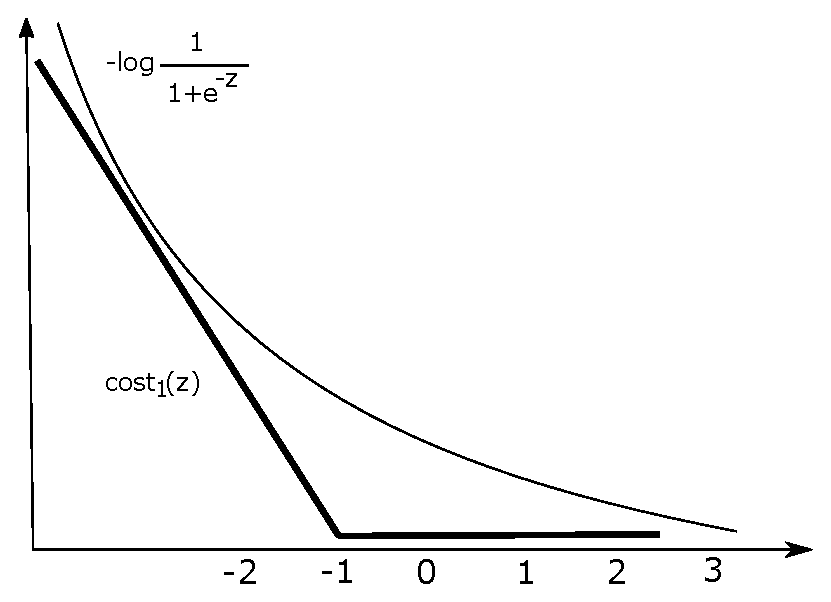
\includegraphics[width=.8\linewidth]{ml_images/cost_1_approx}
\end{minipage}\hfill
\begin{minipage}{0.48\textwidth}
 \centering
 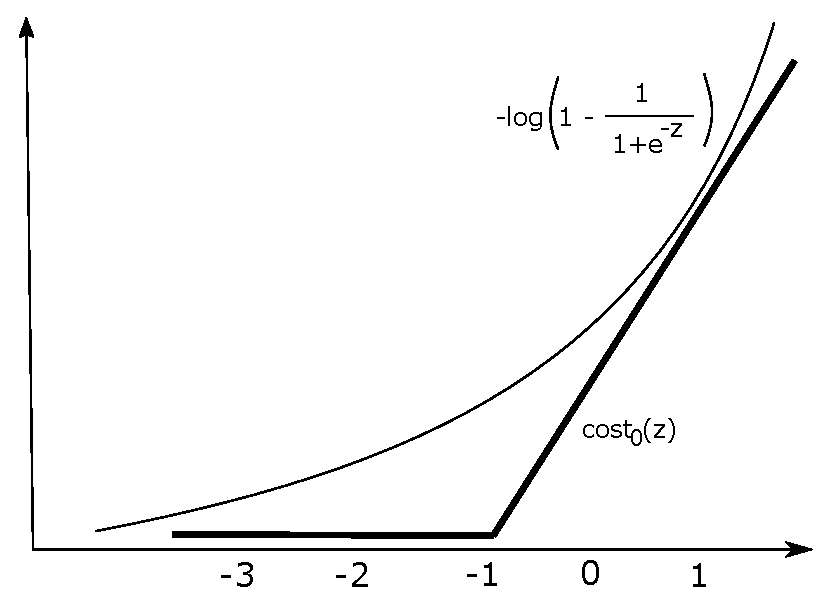
\includegraphics[width=.8\linewidth]{ml_images/cost_0_approx}
\end{minipage}
\end{center}

More precisely, we modify $\text{cost}_1(z)$ so that when $z = \theta^Tx$ is greater than 1, it outputs 0. Furthermore, for values of $z$ less than 1, we use a straight decreasing line instead of the sigmoid curve.
Similarly, we modify $\text{cost}_0(z)$ so that when $z$ is less than -1, it outputs 0. Again, for values of $z$ greater than -1, we use a straight increasing line instead of the sigmoid curve.

Formally, we can define $\text{cost}_0(z)$ and $\text{cost}_1(z)$ as follows (they are also called hinge loss functions):
\begin{equation}\label{eq:hinge-loss}
\begin{split}
\text{cost}_0(z) = \text{max}(0,k(1+z)),\\
\text{cost}_1(z) = \text{max}(0,k(1−z)),
\end{split}
\end{equation}
where $k$ is a constant defining the magnitude of the slope of the line.

Putting all these together, we define the regularized cost function for SVM by
\begin{equation}\label{eq:svm-cost}
J(\theta) = C\displaystyle\sum_{i=1}^m \left[y^{i}\text{cost}_1(z^{i}) + (1 - y^{i})\text{cost}_0(z^{i})\right] + \dfrac{1}{2}\sum_{j=1}^n \theta^2_j.
\end{equation}

This definition of $J(\theta)$ is the same as the corresponding definition \ref{eq:log-reg-costreg} for regularized logistic regression, up to some minor changes. First of all, $\text{cost}_0(z)$ and $\text{cost}_1(z)$ are the ones given by the formula \ref{eq:hinge-loss}. Then we multiply by $m$ (the training set size), since this does not affect the optimization result. Furthermore, for the regularization part we use a large constant $C$ instead of $\lambda$ (this is equivalent to multiplying the equation by $C = \dfrac{1}{\lambda}$). Now, to reduce overfitting, we can decrease $C$, and to reduce underfitting, we can increase $C$.

With these changes, the hypothesis $h_\theta$ of the SVM becomes a discriminant function, i.e. it outputs either 1 or 0. This is different from logistic regression, where the hypothesis outputs the probability of $y$ being 1 or 0. Actually, we have that $h_\theta(x) = 1$ if $\theta^Tx \ge 1$ and $h_\theta(x) = 0$ if $\theta^Tx \le -1$, which makes SVM to be a large margin classifier (see the figure below).

\hspace{1.0in}
\begin{center}
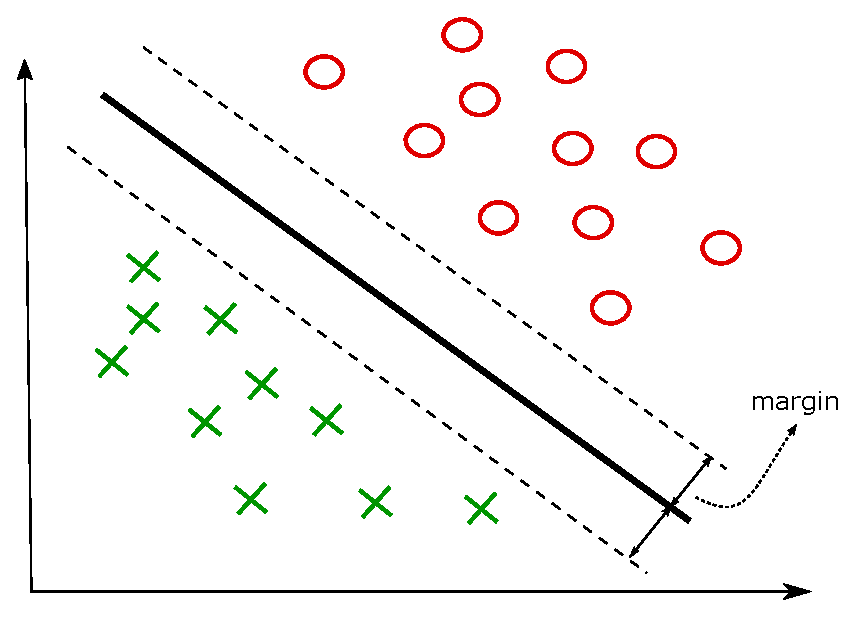
\includegraphics[height = 1.8in]{ml_images/svm}
\end{center}

In SVM, the decision boundary has the special property that it is as far away as possible from both the positive and the negative examples. The distance from the decision boundary to the nearest example is called the margin. Since SVM maximizes this margin, it is often described as a large margin classifier. Notice that a large margin is only achieved when the regularization constant $C$ is very large. Thus, if we have outliers that can affect the decision boundary, we can reduce $C$.


\section{SVM with non-linear kernel}

Kernels allow us to make complex, non-linear classifiers using SVM.

Given a training example $x$, we choose some landmark $l^{1}, l^{2}, \ldots, l^{k}$ in the training space and compute new features depending on the proximity to these landmarks. To do this, we define the similarity $f_j$ of $x$ and $l^{j}$ by using the Gaussian kernel function
$$f_j = \ds\exp\left(-\frac{\norm{x - l^{j}}^2}{2\sigma^2}\right),$$
where $\sigma$ is a parameter of the Gaussian kernel.

Observe that if $x$ is very close to a landmark $l^{j}$, then the corresponding similarity $f_j$ is very close to 1. On the other hand, if $x$ is far away from $l^{j}$, then $f_j$ is close to 0. Thus, one can say that $f_j$ measures how far is $x$ from the landmark $l^{j}$.

Since each landmark provides us with a new feature, we can define a new hypothesis $h_\theta$ by
$$h_\theta(x) = \theta_0 + \ds\sum_{j=1}^{k}{\theta_j f_j},$$
and predict $y=1$ if $h_\theta(x) \ge 0$ and $y=0$ if $h_\theta(x) < 0$.

Notice that choosing a particular set of landmarks defines the shape of the decision boundary, as in the following figure.

\hspace{1.0in}
\begin{center}
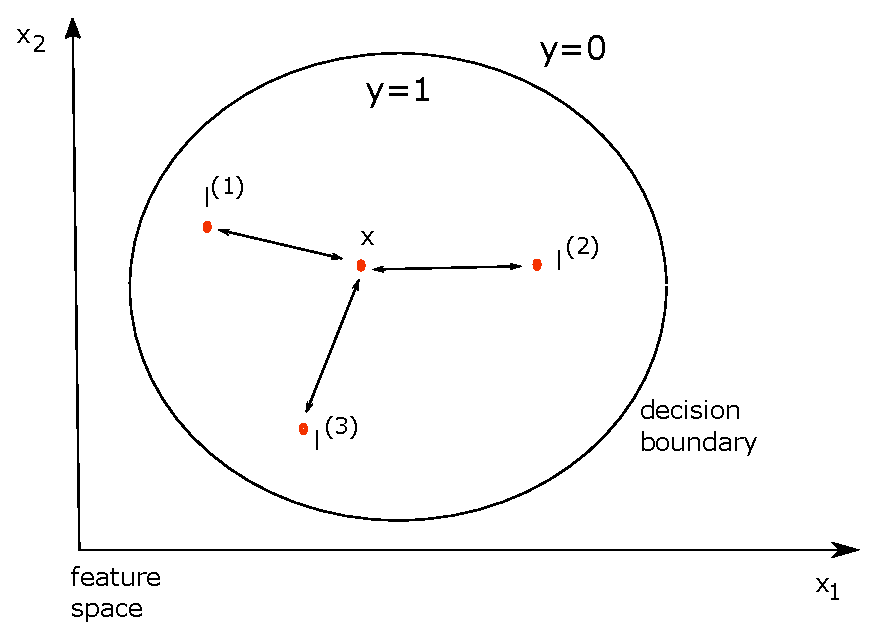
\includegraphics[height = 1.8in]{ml_images/kernel}
\end{center}

We can choose the landmarks to be exactly the training examples. Given a training set $(x^1, y^1), \ldots, (x^m, y^m)$, take $l^{j} = x^j$, and define the features $f_j$ as above, for all $j=1, \ldots, m$.

Each training example $(x^i, y^j)$ defines a vector of features $f^i = [f^i_0, f^i_1, \ldots, f^i_m]^T \in \mathbb{R}^{m+1}$, where $f^i_0 = 1$ and $f^i_j$ is the similarity between $x^i$ and $l^j$.

Then, given a new input $x$ we compute the corresponding feature vector $f\in\mathbb{R}^{m+1}$ and predict $y=1$ if $\theta^Tf \ge 0$  and $y=0$ if $\theta^Tf < 0$, where the parameters vector $\theta$ minimizes the following SVM cost function:
$$ J(\theta) = C\sum_{i=1}^m \left[y^{i}\text{cost}_1(\theta^Tf^{i}) + (1 - y^{i})\text{cost}_0(\theta^Tf^{i})\right] + \dfrac{1}{2}\sum_{j=1}^n \theta^2_j.$$

A very large value of $C$ implies overfitting (low bias, high variance), while a very small value of $C$ implies underfitting (high bias, low variance).

Using kernels to generate features is not exclusive to SVM and may also be applied to logistic regression. However, kernels combined with SVM are much faster comparing with other algorithms.


\subsubsection*{How to use a SVM}

To use a SVM in practice, we have to choose
\begin{itemize}
\item the regularization parameter $C={1}/{\lambda}$:
\begin{itemize}
  \item if $C$ is large, then we have higher variance/lower bias,
  \item If $C$ is small, then we have lower variance/higher bias,
\end{itemize}
\item the kernel (similarity function)
\begin{itemize}
\item no kernel (or linear kernel) - gives a standard linear classifier, works well when $n$ is large and when $m$ is small,
\item Gaussian Kernel - needs feature scaling and a choice of $\sigma^2$, works well when $n$ is small and $m$ is large.
\end{itemize}
\end{itemize}

We can optimize $C$ and the kernel parameters using a cross-validation set.

Notice that not all the similarity functions are valid kernels (they must satisfy a technical condition for convergence called Mercer's theorem).

SVM can be used for multiclass classification with the one-vs-all method we used for logistic regression. If there are $k$ different classes, then we train $k$ SVMs with parameters $\theta^1, \theta^2, \ldots, \theta^k$ and, for an input $x$, we pick the class $j$ with the largest $(\theta^i)^Tx$.

\subsubsection*{Logistic regression vs. SVM}

\begin{itemize}
  \item if the number of features $n$ is large (relative to the number of training examples $m$), use logistic regression or SVM with linear kernel (they are very similar),
  \item if $n$ is small and $m$ is intermediate, use SVM with Gaussian kernel,
  \item if $n$ is small and $m$ is large, create more features and used linear methods.
\end{itemize}

A neural network is likely to work well for all these cases, but may be slower to train.


\chapter{Unsupervised Learning}

Unsupervised learning is opposite to supervised learning because it uses unlabeled data rather than labeled data. In other words, there is no vector $y$ of expected prediction, but only a dataset of features where we need to find structure.

\section{Clustering: K-Means Algorithm}

Clustering refers to the task of grouping a set of data points in such a way that points in the same group (called cluster) are more similar, in a particular sense, to each other than to those in other groups. The k-means algorithm is the most popular and widely used algorithm for solving such a problem.

Assume that we have an unlabeled dataset $x^1, \ldots, x^m \in \mathbb{R}^n$ that we want to group in $K$ different clusters ($K < m$).

\subsubsection*{The steps of k-means}

\begin{description}
  \item[Initialization] Randomly initialize $K$ points, called cluster centroids, $\mu_1, \mu_2, \ldots, \mu_K\ \in \mathbb{R}^n$.
  \item[Clusters assignment] Assign all training examples into one of the groups based on which centroid the example is closest to and record the cluster index:
  $$c^{(i)} := \text{argmin}_{k}{\norm{x^i - \mu_k}^2}\; ; \; i=1,\ldots,m. $$
  \item[Move centroids] Compute the averages of all the points inside each cluster, then move the cluster centroid points to those averages:
  $$\mu_k := \text{average of } \{x^i \;|\; c^{(i)} = k\}\; ; \; k=1,\ldots,K.$$
  \item[Convergence] Repeat the previous step until the centroids do not move anymore.
\end{description}

We can formally define a cost function for the K-means algorithm (also called distortion):
$$J(c, \mu) = \dfrac{1}{m} \sum_{i=1}^{m}{\norm{x^i - \mu_{c^{(i)}}}^2},$$ where $c = (c^{(1)}, \ldots, c^{(m)})$ and $\mu = (\mu_1, \ldots, \mu_K)$.
Then the objective of the algorithm is to minimize $J(c, \mu)$ in terms of $c$ (cluster assignment) and $\mu$ (move centroids).

Remark that it is not possible for the cost function $J(c, \mu)$ to increase, it should descend at each step.

K-means algorithm can get stuck in local optima of $J(c, \mu)$, depending on the initial centroids assignment. We can try many different random initializations and choose the one with the lowest distortion (it is strongly recommended to do this when $K<10$). We also need to make sure that $K < m$ and that the initial centroids are unique.

If there is no clue on how to choose the number of clusters, we can automatically do that by doing an elbow analysis.  The cost function should decrease as we increase the number of clusters, and then flatten out. Choose $K$ at the point where the cost function starts to flatten out. However, fairly often, the curve is very gradual, so there's no clear elbow. The cost function $J$ will always decrease as $K$ increases. The one exception is if $K$-means gets stuck at a bad local optimum.

\hspace{1.0in}
\begin{center}
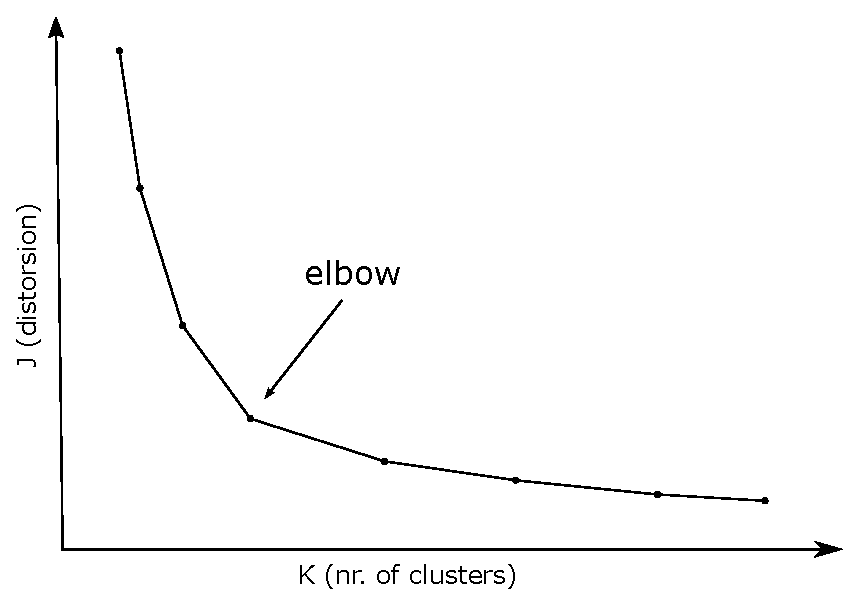
\includegraphics[height = 1.8in]{ml_images/elbow}
\end{center}

Another way to choose $K$ is to observe how well $K$-means performs on a downstream purpose. In other words, we can choose $K$ that proves to be most useful for the goal we are trying to achieve by using these clusters.


\section{Dimensionality reduction: PCA}

We may want to reduce the dimension of the features if we have a lot of redundant data. Doing dimensionality reduction will reduce the total data we have to store in memory and will speed up the learning algorithm.

In dimensionality reduction, we are reducing the number of features rather than the number of examples. The dataset size $m$ will stay the same, but $n$, the number of features, will be reduced.

Another motivation for dimensionality reduction may be data visualization. It is not easy to visualize data that is more than three dimensions. We can reduce the dimensions of our data to 3 or less in order to plot it.

\subsection*{Principal component analysis}

The most popular dimensionality reduction algorithm is Principal Component Analysis (PCA). For example, given two features, we want to find a single feature that effectively describes both features at once. We then map our old features onto this new feature to reduce their number from two to one. The same can be done with three features, where we map them to a 2-dimensional plane.

The goal of PCA is to reduce the feature space from $n$ dimensions to $k$ dimensions, where $k < n$. To do this, we find a $k$-dimensional space onto which to project the data in such a way that the (orthogonal) projection error is minimal. More precisely, we find $k$ vectors $u^1, u^2, \ldots, u^k$ and take their linear span to project onto.

Assume that we have a training set $\{x^1, x^2, \ldots, x^m\}$ of $n$-dimensional vectors. Before doing PCA, we must do some data pre-processing (feature scaling/mean normalization), since we want all the features to have comparable range of values.

For each feature $x_j$, define $\mu_j = \dfrac{1}{m}\ds\sum_{i=1}^{m}{x^i_j}$ and let $s_j$ be either the standard deviation or the difference between max and min. Then replace each $x_j^i$ by $x_j^i = \dfrac{x_j^i - \mu_j}{s_j}$.

After the data pre-processing step, we compute the covariance matrix of the initial dataset: $$\Sigma = \dfrac{1}{m} \ds\sum_{i=1}^{m}{x^i(x^i)^T}.$$
Notice that $x^i$ is an $(n\times 1)$-dimensional vector and $(x^i)^T$ is an $(1\times n)$-dimensional vector, thus $\Sigma$ is an $(n\times n)$-dimensional matrix.

Then we compute the eigenvectors $U = [u^1, u^2, \ldots, u^n]$ of $\Sigma$, which are vectors in $\mathbb{R}^n$ since $\Sigma$ is a symmetric semi-positive definite matrix. To reduce our initial $n$-dimensional feature space, we keep only the first $k$ eigenvectors $U_\text{pr} = [u^1, u^2, \ldots, u^k]\in\mathbb{R}^{n\times k}$, $k<n$, called principal components. Then, for each $i=1,\ldots, m$, we define the reduced features
$$z^i := U_\text{pr}^T x^i \in \mathbb{R}^k.$$
Once we use PCA to compress the data, we can always reconstruct back the initial features. Then we get back the approximations of out initial features $$x_{\text{approx}}^i = Uz^i,$$ where $U$ is the matrix of all eigenvalues of $\Sigma$.


There is one problem remaining, how do we choose k, the number of principal components? One way we do this in practice is to choose $k$ to be the smallest value so that
$$\dfrac{\frac{1}{m}\sum_{i=1}^{m}{\norm{x^i - x_{\text{approx}}^i}^2}}{\frac{1}{m}\sum_{i=1}^{m}{\norm{x^i}^2}} \leq 0.01$$
In other words, the squared projection error divided by the total variation in data should be less than 1\%, so that 99\% of the variance is retained.

The most common use of PCA is to speed up supervised learning algorithms. Given a training set with a large number of features $\{x^i\in\mathbb{R}^n, y^i\}$, we use PCA to obtain a new training set $\{z^i\in\mathbb{R}^k, y^i\}$, where $k<n$. Mapping $x^i$ onto $z^i$ should be learned only on the training set and then used on test, validation sets, etc.

It is a bad practice to use PCA for feature selection or overfitting prevention since the dimensionality reduction doesn't use the labels (use regularization instead). Do not assume that you need dimensionality reduction, just try the full algorithm first and then use dimensionality reduction to speed up the training.


\chapter{Applied ML}

\section{Anomaly detection}

\subsection*{Build anomaly detectors}

Anomaly detection is a popular learning algorithm used in fraud detection, manufacturing, system monitoring, etc.

Assume we have a dataset $\{x^1, x^2,\ldots, x^m\}\in \mathbb{R}^n$ and, for any new example $x_{test}$, we want to know whether this new example is abnormal/anomalous (e.g. fraud, manufacturing defect, system error, etc.).

We define a model $p(x)$ that tells us the probability that the example is not anomalous. We also use a threshold $\varepsilon$ as a dividing line so we can say which examples are anomalous and which are not.
If the detector is flagging too many anomalous examples, then we need to decrease the threshold $\varepsilon$.

Recall the normal (Gaussian) distribution $\mathcal{N}(\mu, \sigma^2)$ density function
$$p(x) = \dfrac{1}{\sigma\sqrt{2\pi}} \exp\left(-\dfrac{(x-\mu)^2}{2\sigma^2}\right).$$

IN general, $\{x^1, x^2,\ldots, x^m\}$ are normally distributed $\mathcal{N}(\mu, \sigma^2)$. We can estimate $\mu$ from data by taking the sample mean
$$\mu = \dfrac{1}{m} \ds\sum_{i=1}^{m}{x^i},$$
and $\sigma^2$ by taking the sample variance
$$\sigma^2 = \dfrac{1}{m} \ds\sum_{i=1}^{m}{(x^i - \mu)}^2.$$

To estimate the density function $p(x)$ on the training set $\{x^1, x^2,\ldots, x^m\}$, we assume that the features $x_j$ are normally distributed $\mathcal{N}(\mu_j, \sigma_j^2)$ (the features should not be necessarily independent, but the algorithm works better of they are).

We first estimate the parameters $\mu_j$ and $\sigma_j^2$ as above
$$\mu_j = \dfrac{1}{m} \ds\sum_{i=1}^{m}{x_j^i}  \; ; \;\;\;  \sigma_j^2 = \dfrac{1}{m} \ds\sum_{i=1}^{m}{(x_j^i - \mu_j)}^2.$$

Then we define $p(x)$ as the product of the feature densities
$$ p(x) := \ds\prod_{j=1}^{n}{p(x_j; \mu_j, \sigma_j^2)} = \prod_{j=1}^{n}\dfrac{1}{\sigma_j\sqrt{2\pi}} \exp\left(-\dfrac{(x_j-\mu_j)^2}{2\sigma_j^2}\right).$$

Thus, whenever we have a new example $x$, we compute $p(x)$ and say that $x$ is an anomaly if $p(x) < \varepsilon$, for a small threshold $\varepsilon$.

\subsection*{Evaluate anomaly detectors}

To evaluate an anomaly detector, we take a labeled data set, categorized into anomalous and non-anomalous examples ($y = 0$ if normal and $y = 1$ if anomalous). Take a large proportion of good, non-anomalous data from the training set on which to train $p(x)$. Then, take a smaller proportion of mixed anomalous and non-anomalous examples (you will usually have many more non-anomalous examples) for your cross-validation and test sets. For example, we may have a set where 0.2\% of the data is anomalous. We take 60\% of those examples, all of which are good ($y=0$) for the training set. We then take 20\% of the examples for the cross-validation set (with 0.1\% of the anomalous examples) and another 20\% from the test set (with another 0.1\% of the anomalous). In other words, we split the data 60/20/20 training/CV/test and then split the anomalous examples 50/50 between the CV and test sets.

Fit the model $p(x)$ on the training set. On a cross validation/test example $x$, predict: if $p(x) < \varepsilon$ (anomaly), then $y=1$ and if $p(x) ≥ \varepsilon$ (normal), then $y=0$. Possible evaluation metrics: precision/recall, $F_1$ score. We use the cross-validation set to choose parameter $\varepsilon$.

\subsection*{Anomaly detection vs. supervised learning}

Use anomaly detection when:
\begin{itemize}
\item We have a very small number of positive examples ($y=1$: 0-20 examples is common) and a large number of negative ($y=0$) examples.
\item We have many different "types" of anomalies and it is hard for any algorithm to learn from positive examples what the anomalies look like; future anomalies may look nothing like any of the anomalous examples we've seen so far.
\end{itemize}

Use supervised learning when:
\begin{itemize}
\item We have a large number of both positive and negative examples. In other words, the training set is more evenly divided into classes.
\item We have enough positive examples for the algorithm to get a sense of what new positives examples look like. The future positive examples are likely similar to the ones in the training set.
\end{itemize}
Choosing Features

The features will greatly affect how well your anomaly detection algorithm works. We can check that our features are gaussian by plotting a histogram of our data and checking for the bell-shaped curve or by using statistical tests.

Some transformations we can use on features that do not have the bell-shaped curve are: $\log(x)$, $\log(1+x)$, $\sqrt{x}$, $x^{1/3}$. We can play with each of these to achieve the Gaussian shape of the data.
There is an error analysis procedure for anomaly detection that is very similar to the one in supervised learning. Our goal is for $p(x)$ to be large for normal examples and small for anomalous examples.
One common problem is when $p(x)$ is similar for both types of examples. In this case, you need to examine the anomalous examples that are giving high probability in detail and try to figure out new features that will better distinguish the data. In general, choose features that might take on unusually large or small values in the event of an anomaly.


\subsection*{Multivariate Gaussian Distribution}

The multivariate Gaussian distribution is an extension of anomaly detection and may (or may not) catch more anomalies.

Instead of modeling $p(x_1),p(x_2),\ldots, p(x_n)$, separately, we will model $p(x)$ all in one go. Our parameters will be: $\mu \in \mathbb{R}^n$ and $\Sigma\in \mathbb{R}^{n\times n}$ and
$$p(x;\mu,\Sigma) = \dfrac{1}{(2\pi)^{n/2} |\Sigma|^{1/2}} \exp(-1/2(x-\mu)^T\Sigma^{-1}(x-\mu)).$$
The important effect is that we can model oblong Gaussian contours, allowing us to better fit data that might not fit into the normal circular contours.
Varying $\Sigma$ changes the shape, width, and orientation of the contours. Changing $\mu$ will move the center of the distribution.

When doing anomaly detection with multivariate gaussian distribution, we compute $\mu$ and $\Sigma$ from data. We then compute $p(x)$ using the new formula in the previous section and flag an anomaly if $p(x) < \varepsilon$.
The original model for $p(x)$ corresponds to a multivariate Gaussian where the contours of $p(x;\mu,\Sigma)$ are axis-aligned.
The multivariate Gaussian model can automatically capture correlations between different features of $x$.

However, the original model maintains some advantages: it is computationally cheaper (no matrix to invert, which is costly for large number of features) and it performs well even with small training set size (in multivariate Gaussian model, $m$ should be greater than the number of features for $\Sigma$ to be invertible).


\section{Recommender Systems}

\subsection*{Problem Formulation}

Recommendation is currently a very popular application of machine learning.

Say we are trying to recommend movies to customers. We can use the following definitions

$n_u$ = number of users

$n_m$ = number of movies

$r(i,j) = 1$ if user $j$ has rated movie $i$

$y(i,j)$ = rating given by user $j$ to movie $i$ (defined only if $r(i,j)=1$)

\subsection*{Content Based Recommendations}

We can introduce two features, $x_1$ and $x_2$ which represents how much romance or how much action a movie may have (on a scale of 0−1). One approach is that we could do linear regression for every single user. For each user $j$, learn a parameter $\theta(j)\in \mathbb{R}^3$. Predict user $j$ as rating movie $i$ with $(\theta^{(j)})^Tx^{(i)}$ stars.

$\theta^{(j)}$ = parameter vector for user $j$

$x^{(i)}$ = feature vector for movie $i$

For user $j$, movie $i$, predicted rating: $(\theta^{(j)})^T(x^{(i)})$

$m^{(j)}$ = number of movies rated by user $j$

To learn $\theta^{(j)}$, we do the following

$$min_{\theta^{(j)}} = \dfrac{1}{2}\displaystyle \sum_{i:r(i,j)=1} ((\theta^{(j)})^T(x^{(i)}) - y^{(i,j)})^2 + \dfrac{\lambda}{2} \sum_{k=1}^n(\theta_k^{(j)})^2$$

This is our familiar linear regression. The base of the first summation is choosing all $i$ such that $r(i,j) = 1$.

To get the parameters for all our users, we do the following:

$$min_{\theta^{(1)},\dots,\theta^{(n_u)}} = \dfrac{1}{2}\displaystyle \sum_{j=1}^{n_u} \sum_{i:r(i,j)=1} ((\theta^{(j)})^T(x^{(i)}) - y^{(i,j)})^2 + \dfrac{\lambda}{2} \sum_{j=1}^{n_u} \sum_{k=1}^n(\theta_k^{(j)})^2$$

We can apply our linear regression gradient descent update using the above cost function. The only real difference is that we eliminate the constant $\dfrac{1}{m}$.

\subsection*{Collaborative Filtering}

It can be very difficult to find features such as "amount of romance" or "amount of action" in a movie. To figure this out, we can use feature finders.

We can let the users tell us how much they like the different genres, providing their parameter vector immediately for us.

To infer the features from given parameters, we use the squared error function with regularization over all the users:

$$min_{x^{(1)},\dots,x^{(n_m)}} \dfrac{1}{2} \displaystyle \sum_{i=1}^{n_m} \sum_{j:r(i,j)=1} ((\theta^{(j)})^T x^{(i)} - y^{(i,j)})^2 + \dfrac{\lambda}{2}\sum_{i=1}^{n_m} \sum_{k=1}^{n} (x_k^{(i)})^2$$

You can also randomly guess the values for theta to guess the features repeatedly. You will actually converge to a good set of features.

To speed things up, we can simultaneously minimize our features and our parameters:

$$J(x,\theta) = \dfrac{1}{2} \displaystyle \sum_{(i,j):r(i,j)=1}((\theta^{(j)})^Tx^{(i)} - y^{(i,j)})^2 + \dfrac{\lambda}{2}\sum_{i=1}^{n_m} \sum_{k=1}^{n} (x_k^{(i)})^2 + \dfrac{\lambda}{2}\sum_{j=1}^{n_u} \sum_{k=1}^{n} (\theta_k^{(j)})^2$$

It looks very complicated, but we've only combined the cost function for $\theta$ and the cost function for $x$.

Because the algorithm can learn them itself, the bias units where $x_0=1$ have been removed, therefore $x\in\mathbb{ℝ}^n$ and $\theta \in\mathbb{ℝ}^n$.

These are the steps in the algorithm:
\begin{itemize}
\item Initialize $x^{(i)},...,x^{(n_m)},\theta^{(1)},...,\theta^{(n_u)}$ to small random values. This serves to break symmetry and ensures that the algorithm learns features $x^{(i)},...,x^{(n_m)}$ that are different from each other.
\item Minimize $J(x^{(i)},...,x^{(n_m)},\theta^{(1)},...,\theta^{(n_u)})$ using gradient descent (or an advanced optimization algorithm). E.g. for every $j=1,...,n_u, i=1,...,n_m$:
$$x_k^{(i)} := x_k^{(i)} - \alpha\left (\displaystyle \sum_{j:r(i,j)=1}{((\theta^{(j)})^T x^{(i)} - y^{(i,j)}) \theta_k^{(j)}} + \lambda x_k^{(i)} \right)$$
​$$\theta_k^{(j)} := \theta_k^{(j)} - \alpha\left (\displaystyle \sum_{i:r(i,j)=1}{((\theta^{(j)})^T x^{(i)} - y^{(i,j)}) x_k^{(i)}} + \lambda \theta_k^{(j)} \right)$$
\item For a user with parameters $\theta$ and a movie with (learned) features $x$, predict a star rating of $\theta^Tx$.
​\end{itemize}​	

\subsection*{Low Rank Matrix Factorization}

Given matrices $X$ (each row containing features of a particular movie) and $\Theta$ (each row containing the weights for those features for a given user), then the full matrix $Y$ of all predicted ratings of all movies by all users is given simply by: $Y=X\Theta^T$.

Predicting how similar two movies $i$ and $j$ are can be done using the distance between their respective feature vectors $x$. Specifically, we are looking for a small value of $\norm{x^{(i)} - x^{(j)}}$.

Mean Normalization

If the ranking system for movies is used from the previous lectures, then new users (who have watched no movies), will be assigned new movies incorrectly. Specifically, they will be assigned $\theta$ with all components equal to zero due to the minimization of the regularization term. That is, we assume that the new user will rank all movies 0, which does not seem intuitively correct.

We rectify this problem by normalizing the data relative to the mean. First, we use a matrix $Y$ to store the data from previous ratings, where the $i$-th row of $Y$ is the ratings for the $i$-th movie and the $j$-th column corresponds to the ratings for the $j$-th user.

We can now define a vector $\mu = [\mu_1, \mu_2, \dots , \mu_{n_m}]$ such that $$\mu_i = \frac{\sum_{j:r(i,j)=1}{Y_{i,j}}}{\sum_{j}{r(i,j)}}$$

Which is effectively the mean of the previous ratings for the $i$-th movie (where only movies that have been watched by users are counted). We now can normalize the data by subtracting $u$, the mean rating, from the actual ratings for each user (column in matrix $Y$):

As an example, consider the following matrix $Y$ and mean ratings $\mu$:

$$Y =
\begin{bmatrix}
    5 & 5 & 0 & 0  \\
    4 & ? & ? & 0  \\
    0 & 0 & 5 & 4 \\
    0 & 0 & 5 & 0 \\
\end{bmatrix},
\quad
 \mu =
\begin{bmatrix}
    2.5 \newline
    2  \newline
    2.25 \newline
    1.25 \newline
\end{bmatrix}$$

The resulting $Y^\prime$ vector is:

$$Y' =
\begin{bmatrix}
  2.5    & 2.5   & -2.5 & -2.5 \\
  2      & ?     & ?    & -2 \\
  -.2.25 & -2.25 & 3.75 & 1.25 \\
  -1.25  & -1.25 & 3.75 & -1.25
\end{bmatrix}$$

Now we must slightly modify the linear regression prediction to include the mean normalization term:

$$(\theta^{(j)})^T x^{(i)} + \mu_i$$

Now, for a new user, the initial predicted values will be equal to the $\mu$ term instead of simply being initialized to zero, which is more accurate.

















\end{document}
